% Forum abbreviations (to insert in \documentclass options): 
% Atmospheric Chemistry and Physics Discussions 	acpd 
% Atmospheric Measurement Techniques Discussions 	amtd 
% Biogeosciences Discussions 	bgd 
% Climate of the Past Discussions 	cpd 
% Drinking Water Engineering and Science Discussions 	dwesd 
% Earth System Dynamics Discussions 	esdd 
% Earth Surface Dynamics Discussions 	esurfd 
% Earth System Science Data Discussions 	essdd 
% Geoscientific Instrumentation, Methods and Data Systems Discussions 	gid 
% Geoscientific Model Development Discussions 	gmdd 
% Hydrology and Earth System Sciences Discussions 	hessd 
% Natural Hazards and Earth System Sciences Discussions 	nhessd 
% Ocean Science Discussions 	osd 
% Solid Earth Discussions 	sed 
% The Cryosphere Discussions 	tcd 

\documentclass[hvmath, online,bgd]{copernicus_discussions}
\usepackage{xcolor}
\usepackage{hyperref}
\usepackage{adjustbox}
\usepackage{natbib}

\begin{document}

%\linenumbers

\title{What controls the variability of CO$_{2}$ fluxes in eastern boundary upwelling systems?}

\author[1]{Riley X. Brady}
\author[1]{Nicole S. Lovenduski}
\author[2]{Michael A. Alexander}
\author[3]{Michael Jacox}
\author[4]{Nicolas Gruber}

\affil[1]{Department of Atmospheric and Oceanic Sciences and Institute of Arctic and Alpine Research, University of Colorado, Boulder, CO, USA}
\affil[2]{NOAA/ESRL, Boulder, CO, USA}
\affil[3]{University of California, Santa Cruz, CA and NOAA/SWFSC, Monterey, CA, USA}
\affil[4]{Environmental Physics, Institute of Biogeochemistry and Pollutant Dynamics, ETH Z\"urich, Z\"urich, Switzerland}

\runningtitle{Sample Title}
\runningauthor{Author Name}

\correspondence{Riley X. Brady (riley.brady@colorado.edu)}


\firstpage{1}

\maketitle  

\begin{abstract}
Eastern Boundary Upwelling Systems (EBUS) are governed by alongshore, equatorward winds that force cold, corrosive, and nutrient-enriched waters to the surface. The complex physical and biological dynamics of these regions leads to a temporally variable mosaic of air-sea CO$_{2}$ fluxes with some of the highest flux densities globally. This variability can dictate when we might expect the anthropogenic signal of CO$_2$ flux to become emergent in each system. In this study, we diagnose the physical and biological mechanisms that control historical (1920-2015) CO$_{2}$ fluxes in the four major EBUS: the California (CalCS), Humboldt (HumCS), Canary (CanCS), and Benguela Currents (BenCS). We utilize biogeochemical output from the CESM Large Ensemble, a global coupled climate model ensemble that is forced under historical and RCP8.5 radiative forcing. Differences between simulations can be attributed entirely to internal climate variability, as simulations are generated by introducing round-off perturbations to the initial atmospheric temperature. This experimental setup provides us with 34 independent and unique representations of the natural climate system, allowing us to robustly assess variability in CO$_{2}$ fluxes. We find that anomalous CO$_{2}$ flux in the CalCS and CanCS is most associated with oscillations in oceanic and atmospheric subtropical gyres: the North Pacific Gyre Oscillation (NPGO) and the North Atlantic Oscillation (NAO), respectively. The CalCS (CanCS) has anomalous uptake (outgassing) of carbon during the positive phase of the NPGO (NAO). The HumCS responds mainly to El Ni\~no Southern Oscillation (ENSO), with anomalous uptake of CO$_{2}$ during an El Ni\~no event. Variations in dissolved inorganic carbon (DIC) and sea surface temperatures (SST) are the major contributors to these anomalous fluxes, and are generally driven by changes to upwelling, the mixed layer depth, and biology. A better understanding of the sensitivity of CO$_{2}$ fluxes in EBUS to internal climate variability might lead to some short-term predictive skill in the ocean--atmosphere carbon cycle. Skillful prediction would be particularly useful in forecasting and managing the onset of ocean acidification in systems that have a naturally low pH and carbonate ion concentration.
\end{abstract}



\introduction[Introduction]  %% \introduction[modified heading if necessary]
The four major Eastern Boundary Upwelling Systems (EBUS) occur at the eastern edges of subtropical gyres in the Atlantic and Pacific oceans -- the California Current System (CalCS), Humboldt Current System (HumCS), Canary Current System (CanCS), and Benguela Current System (BenCS). These regions are characterized by semi-permanent or permanent equatorward winds that drive both coastal Ekman upwelling and curl-driven Ekman pumping within the first 200km of the coastline \citep{Chavez:2009}. Upwelling delivers deep waters with respired nutrients to the surface, fueling fisheries that are highly productive with respect to the small surface area they cover \citep{Ryther:1969}. This process also supplies waters with an elevated dissolved inorganic carbon (DIC) content, which enhances the partial pressure of carbon dioxide (\textit{p}CO$_{2}$) and reduces the pH and carbonate ion concentration. In turn, these systems are naturally sensitive to the impacts of ocean acidification \citep{Hauri:2009,Bakun:2015,Chan:2017}. 

The carbonate chemistry of EBUS is controlled by a complex interplay of physical and biological processes: entrainment of subsurface waters, horizontal advection, upwelling and vertical mixing, temperature changes, photosynthesis, respiration, and calcium carbonate formation and dissolution \citep{DeGrandpre:1998, King:2007}. These terms combine to dictate oceanic \textit{p}CO$_{2}$, which drives the \textit{p}CO$_{2}$ gradient between the ocean and atmosphere ($\Delta$\textit{p}CO$_{2}$), thus contributing to the magnitude and determining the direction of air-sea CO$_{2}$ fluxes. 

Although coastal oceans around the world have small contributions to the global carbon flux, they are characterized by a high CO$_{2}$ flux density, or the magnitude of air-sea carbon exchange per unit area \citep{Laruelle:2010,Laruelle:2014,Gruber:2015}. Low-latitude upwelling systems, such as the HumCS and CanCS, tend to be net outgassing systems, due to their relatively warm waters and persistent upwelling. Because of their colder temperatures and active biology, mid-latitude systems, such as the CalCS and BenCS, act as weak CO$_{2}$ sinks that can become CO$_{2}$ sources during certain seasons \citep{Borges:2002,Hales:2005,Cai:2006,Gregor:2013}. Surface ocean \textit{p}CO$_{2}$ and thus air-sea CO$_2$ flux in EBUS exhibits high temporal variability at sub-seasonal, seasonal, and interannual time scales \citep{Friederich:2002,Gonzales:2009,Leinweber:2009, Evans:2011,Turi:2014}. Although the pronounced temporal variability of CO$_{2}$ fluxes in EBUS has been documented by a number of studies, little work has been done to associate it directly with internal climate variability. 

It has long been recognized that EBUS have intense variations in biology that are coupled to large-scale physical variability \citep[\textit{e.g.},][]{Chelton:1982, Barber:1983, Barber:1986}. Studies have associated this variability with major climate indices, such as the El Ni\~no Southern Oscillation \citep[ENSO;][]{Barber:1983,Barber:1986,Lynn:2002,Chavez:2002,Escribano:2004,Frischknecht:2015}, Pacific Decadal Oscillation \citep[PDO;][]{Mantua:1997, Chhak:2007, Chenillat:2012}, North Pacific Gyre Oscillation \citep[NPGO;][]{DiLorenzo:2008, DiLorenzo:2009, Chenillat:2012}, and North Atlantic Oscillation \citep[NAO;][]{Borges:2003,Cropper:2014}. A similar analysis for EBUS CO$_{2}$ fluxes is necessary for the community. Identifying robust relationships between modes of climate variability and CO$_{2}$ fluxes would (1) advance our understanding of the complex carbonate system in EBUS and (2) provide some level of predictability in CO$_{2}$ flux anomalies. EBUS are naturally sensitive to ocean acidification and  have internal variability that rivals the magnitude of the seasonal cycle. 
Thus, forecasting anomalous CO$_{2}$ fluxes could aid in detecting the early onset of seasonal ocean acidification \citep{Landschuetzer:2018,Kwiatkowski:2018,Hauck:2018}.

Previous studies have utilized observations \citep[\textit{e.g.},][]{Boyd:1987,Friederich:2002,Chavez:2002,Santana-Casiano:2007,DiLorenzo:2008,DiLorenzo:2009}  and output from high-resolution hindcast simulations \citep{Jacox:2015,Frischknecht:2015,Frischknecht:2017,Turi:2017,Mogollon:2017} to explore the relationship between climate variability and EBUS biogeochemistry. However, single realizations, whether modeled or observed, provide a limited sample size of internal variability. At most, hindcast model runs and observational time series capture 10 El Ni\~no and 10 La Ni\~na events, and only 1 phase of the PDO. This is problematic, because mid-latitude atmospheric noise can obscure the signal of climate modes such as ENSO, causing a diversity of responses in EBUS \citep{Deser:2017,Deser:2018}. Thus, one requires many more case studies to robustly assess the response of EBUS biogeochemistry to internal variability. A solution to this problem is to use a single-model ensemble that is derived by introducing perturbations to the initial state of the climate system. This gives rise to a set of realizations with unique representations of internal climate variability and gives one access to many hundred ENSO events, rather than just a handful. By performing historical experiments with increasing atmospheric CO$_{2}$ rather than a long control run, we can account for variability in anthropogenic CO$_{2}$ in the ocean as well as potential modifications to the frequency and amplitude of internal variability with climate change \citep[e.g.,][]{Timmermann:1999, Kuzmina:2005, Sydeman:2013, Cai:2014, Cai:2015}. 

In this study, we utilize output from the single-model Community Earth System Model ``Large Ensemble'' \citep[CESM-LENS;][]{Kay:2015,Lovenduski:2016} to identify major modes of climate variability that are associated with anomalous CO$_{2}$ fluxes in the major EBUS. We expand on this by investigating the physical and biological drivers that underpin these anomalies. The single-model ensemble is necessary for such an analysis, since the forced signal can be removed to generate residual simulations that solely represent CO$_{2}$ flux responses to internal climate variability \citep{Thompson:2015}. Since the simulations are forced with historical CO$_{2}$ emissions, each member accounts for the combined response of natural and anthropogenic CO$_{2}$ to climate variability. Furthermore, the availability of 34 simulations allows us to find statistically robust relationships between anomalous fluxes and internal variability. This experimental setup addresses the data limitation issues of an observational study as well as the single realization problem of a model hindcast or a multi-model ensemble.


\section{Methods and Model Evaluation}

\subsection{Model Configuration and Upwelling Regions}
We utilize monthly output from 34 members of the CESM-LENS, which is derived from a fully coupled Atmosphere-Ocean General Circulation Model (AOGCM) with ocean biogeochemistry \citep{Kay:2015,Lovenduski:2016}. Round-off level perturbations are made to the atmospheric temperature in 1920, leading to an ensemble of simulations that diverge solely due to the influence of internally generated variability. This provides us with a set of 34 independent representations of climate variability, with which we can robustly assess the controls on air-sea CO$_{2}$ flux variability in EBUS. The ensemble is forced with historical radiative forcing from 1920--2005 and RCP8.5 radiative forcing from 2006--2100. The ocean model has nominal 1$^{o}$ horizontal resolution with vertical resolution of 10 m through the upper 250 m, thus resolving the Ekman layer. Due to the coarse horizontal resolution, neither curl-driven nor coastal upwelling is directly resolved, but both are represented in the model. A more detailed discussion of coastal upwelling in the CESM-LENS for the CalCS in particular can be found in \cite{Brady:2017}.

Upwelling regions were confined to approximately the 10$^{o}$ latitude of most active upwelling as defined by \citet{Chavez:2009}, although the CanCS domain was shifted north by 9$^{o}$ to capture the more intense upwelling off the Western Sahara in CESM1 (Table~\ref{Table:1}). They were then limited to the first 800km in the offshore direction. The black outlines in Figure~\ref{Fig:Eval}e--h display these regions. The ensemble mean -- which represents both the seasonality and anthropogenic trend for CO$_{2}$ flux -- was removed from each simulation for each upwelling system to create internally generated residuals. All output was analyzed at monthly resolution.

\subsection{Statistical Analysis and Model Equations}
Air-sea CO$_{2}$ fluxes in CESM are computed following the parameterization of \citet{Wanninkhof:2014}:
\begin{equation}
	F = k\cdot K_{0}\cdot\left( pCO_{2}^{o} - pCO_{2}^{a}\right) ,
\end{equation}

\noindent where k represents the gas transfer velocity (dependent on the wind speed squared), K$_{0}$ the solubility of CO$_{2}$ in seawater, and \textit{p}CO$_{2}^{o}$ and \textit{p}CO$_{2}^{a}$ the partial pressures of CO$_{2}$ in the surface ocean and atmosphere, respectively. 

We use a linear Taylor expansion to quantify the relative contribution of each variable to the overall CO$_{2}$ flux anomaly in response  to internally generated variability following \citet{Lovenduski:2007} and \citet{Turi:2014}, 
\begin{equation}
	\Delta F = \frac{\partial F}{\partial U}\Delta U + \frac{\partial F}{\partial pCO_{2}^{oc}}\Delta pCO_{2}^{oc} ,
\end{equation}

\noindent where $\frac{\partial F}{\partial U}$ and $\frac{\partial F}{\partial pCO_{2}^{oc}}$ are determined from the model equations and mean values in each EBUS. $\Delta$'s represent the linear regression of the given variable's residuals onto a climate index. The contributions from $\Delta pCO_{2}^{oc}$ is further decomposed into DIC, Alk, SST, and salinity terms:
\begin{equation}
	\Delta pCO_{2}^{oc} = \frac{\partial pCO_{2}^{oc}}{\partial DIC}\Delta DIC + \frac{\partial pCO_{2}^{oc}}{\partial Alk}\Delta Alk + \frac{\partial pCO_{2}^{oc}}{\partial T}\Delta T + \frac{\partial pCO_{2}^{oc}}{\partial S}\Delta S .
\end{equation}

Because DIC and Alk can be diluted by freshwater fluxes, we introduce salinity-normalized DIC (sDIC) and Alk (sAlk), 
\begin{equation}
	\Delta F = \frac{\partial F}{\partial U}\Delta U + \frac{S}{S_{0}}\frac{\partial F}{\partial DIC}\Delta sDIC + \frac{S}{S_{0}}\frac{\partial F}{\partial Alk}\Delta sAlk + 	\frac{\partial F}{\partial fw}\Delta fw + \frac{\partial F}{\partial T}\Delta T + \frac{\partial F}{\partial S}\Delta S .
\end{equation}

Due to the significance of sDIC anomaly contributions to the total CO$_{2}$ flux anomaly in EBUS, we approximate the mechanisms controlling sDIC anomalies following \cite{Lovenduski:2007},
\begin{equation}
	\frac{d(sDIC^{\prime})}{dt} = J^{\prime}_{circ}+ J^{\prime}_{bio} + J^{\prime}_{ex}
\end{equation}
where $J^{\prime}_{circ}$, $J^{\prime}_{bio}$, and $J^{\prime}_{ex}$ represent the sources and sinks of sDIC$^{\prime}$ from circulation, biology, and CO${2}$ flux anomalies integrated over the upper 100m, respectively. See \citet[][their Equation 4]{Lovenduski:2007} for additional details on these terms and their Appendix B for the computation of $J^{\prime}_{bio}$ in particular. 

To compensate for autocorrelation that is characteristic of climate indices and is also introduced from smoothing, we replace the \textit{t}-statistic sample size \textit{N} with an effective sample size, \textit{N$_{eff}$}:
\begin{equation}
	N_{eff} = N\left(\frac{1 - r_{1}r_{2}}{1 + r_{1}r_{2}}\right)
\end{equation}
where r$_{1}$ and r$_{2}$ are the lag-1 autocorrelation coefficients of the two time series being correlated \citep{Bretherton:1999, Lovenduski:2005}. \textit{N}$_{eff}$ represents the number of statistically independent measurements.

\subsection{Model Evaluation}
CESM-LENS air-sea CO$_{2}$ fluxes were compared to the observationally-based SOM-FFN (Self-Organizing Map-Feed Forward Network) product  from \citet{Landschuetzer:2017} along the four major EBUS outlined by \citet{Chavez:2009}. The SOM-FFN was generated by a two step process. First, the global oceans were grouped into 16 biogeochemical provinces based on common relationships between SSTs, sea surface salinity, mixed layer depth, and \textit{p}CO$_{2}$ climatology from \citet{Takahashi:2009}. Secondly, nonlinear relationships were determined between an expanded set of predictor variables and the Surface Ocean Carbon Atlas version 4 \citep{Bakker:2016} database of surface ocean CO$_{2}$ measurements to interpolate \textit{p}CO$_{2}$ to monthly resolution spanning 1982-2015 at 1$^{o}$x1$^{o}$ global resolution. Extensive details on and validation of the procedure can be found in \citet{Landschuetzer:2013} and \citet{Landschuetzer:2016}.

Figure~\ref{Fig:Eval} compares the historical climatology (1982--2015) between the SOM-FFN (a--d) and the CESM-LENS (e--h). The Pacific systems are particularly well-modeled. The CESM-LENS simulates the meridional gradient of poleward uptake and equatorward outgassing of CO$_{2}$ in the CalCS (Figure~\ref{Fig:Eval}e). For this system and all other EBUS, we do not expect the model to resolve nearshore outgassing, as coastal upwelling here occurs at the sub-grid scale. In the HumCS, the model depicts the strong outgassing that is characteristic of a tropical upwelling system (Figure~\ref{Fig:Eval}f). The CO$_{2}$ flux climatology in the Atlantic systems is more biased in the CESM-LENS. While the SOM-FFN portrays a meridional gradient of relatively weak CO$_{2}$ fluxes in the CanCS, the CESM-LENS simulates strong outgassing along the Western Sahara (Figure~\ref{Fig:Eval}c and g). An important caveat is that the data density of \textit{p}CO$_{2}$ in EBUS informing the SOM-FFN is on the order of the Southern Ocean, a notably undersampled region \citep{Bakker:2016,Laruelle:2017}. In turn, the EBUS CO$_{2}$ fluxes are being informed by remote biogeochemical provinces more often than other regions of the ocean. The BenCS has the most biased CO$_{2}$ flux climatology of the major EBUS in CESM-LENS. Although it simulates the meridional gradient portrayed in the SOM-FFN, the ougassing cell is nearly 10$^{o}$ too far south and is significantly stronger than in the SOM-FFN (Figure~\ref{Fig:Eval}d and h).

The BenCS has the largest physical biases in CESM-LENS than all other EBUS. Its SST bias is in excess of 7$^{o}$C with the nominal 1$^{o}$ atmospheric resolution. Further, it only improves to a 5$^{o}$C bias at 0.5$^{o}$ atmospheric resolution \citep{Gent:2010}. This bias is likely driven by the fact that the Angola-Benguela Front is simulated too far south, in addition to deficiencies in upwelling and meridional transport that are driven by unrealistic alongshore wind stress structure \citep{Small:2015}. Because of these deficiencies that are specific to the BenCS, we will only discuss its internal variability in CO$_{2}$ fluxes in Section 3.1, but will not perform a full analysis on its connections to larger-scale climate variability.

\section{Results}

\subsection{Internal Variability in Upwelling Systems}
We emphasize the magnitude of internal variability in EBUS CO$_{2}$ fluxes in Figure~\ref{Fig:Internal} by showing the ensemble mean standard deviation of air-sea CO$_2$ flux residuals (ensemble mean subtracted) at each location across the global ocean. Save for the Southern Ocean and subpolar Arctic, the EBUS emerge as significant regions influenced by internal variability on a global scale. The HumCS, CanCS, and BenCS in particular have some of the highest internally driven CO$_{2}$ fluxes globally. The CalCS has comparatively low internal variability in CO$_{2}$ fluxes. Coastally, the EBUS are distinct from the major western boundary currents, which appear to be influenced very little by internal variability (Figure~\ref{Fig:Internal}).

Figure~\ref{Fig:TimeSeries} (a--d) displays time series of historical CO$_{2}$ flux from 1920--2015 and the mean seasonal cycle and monthly magnitude of internal variability (e--h) for each of the four EBUS. The black line depicts the seasonal cycle, the red line the anthropogenically forced trend, and the gray shading the component due to internal variability. Values for each of these components and the linear intercept are reported in Table~\ref{Table:1}. The largest absolute internal variability is found in the BenCS and HumCS with values of 0.98 mol~m$^{-2}$~yr$^{-1}$ and 1.20 mol~m$^{-2}$~yr$^{-1}$, respectively (Table~\ref{Table:1}). 
The BenCS is uniquely exposed to variability from the Southern Ocean and Agulhas Current \citep{Reason:2006}. The HumCS likely has intense variability due to its direct connection to the tropical Pacific Ocean and thus rapid communication with ENSO \citep[e.g.,][]{Colas:2008,Montes:2011}. 

All four systems have statistically significant trends toward a greater CO$_{2}$ sink due to the invasion of anthropogenic carbon (Figure~\ref{Fig:TimeSeries}; Table~\ref{Table:1}). This forces the HumCS, CanCS, and BenCS to act as intermittent sinks by 2015 in some realizations due to the combination of the long-term trend and internal variability. The HumCS and BenCS have the largest uptake of anthropogenic CO$_{2}$ over the historical period, which is on the order of the magnitude of their seasonal cycles over the course of 96 years. The CanCS is a unique case, where the anthropogenic trend is more than double the magnitude of its seasonal cycle (Table~\ref{Table:1}). The seasonal cycle of all EBUS excluding the CanCS is approximately sinusoidal with an outgassing peak in the late boreal summer (Figure~\ref{Fig:TimeSeries}e--h). The CanCS has a relatively weak bi-modal outgassing peak in late winter and early summer, but is otherwise relatively flat (Figure~\ref{Fig:TimeSeries}g). It has by far the smallest seasonal cycle of the four systems (Table~\ref{Table:1}). 

The magnitude of internal variability is greater than that of the seasonal cycle for the majority of systems. The non-seasonal component of the total variability (the sum of the seasonal and internal components) is 59\% for the HumCS, 73\% for the CanCS, and 56\% for the BenCS (Table~\ref{Table:1}). Only the CalCS has a stronger seasonal cycle of CO$_{2}$ flux than internal variability, but the non-seasonal component still accounts for 33\% of the variability in this system (Table~\ref{Table:1}). Perhaps for the CalCS, more significant internal variability would be captured at a higher resolution that resolves coastal upwelling, such as in \citet[][Figure~8c]{Turi:2014}. Lastly, internal variability in CO$_{2}$ fluxes tends to be phase-locked with the seasonal cycle for the HumCS and BenCS, as the peak magnitudes of internal variability track the ridges and troughs of the seasonal component (Figure~\ref{Fig:TimeSeries}f and h). The CanCS has more complex behavior in the residuals due to the bi-modal peaks of its seasonal cycle (Figure~\ref{Fig:TimeSeries}g), and the CalCS has a relatively uniform magnitude of internal variability throughout the year (Figure~\ref{Fig:TimeSeries}e).

\subsection{California Current}
Our primary goal for each EBUS was to identify the dominating mode of climate variability associated with its CO$_{2}$ flux residuals. We correlated area-weighted residuals from the black boxes in Figure~\ref{Fig:Eval}e--h for each simulation with every grid cell globally for a set of predictor variables' residuals: SST, sea level pressure (SLP), 10m wind speed, and wind stress curl. We then assessed the ensemble mean of the correlations to determine the mode of climate variability associated with the given global spatial pattern. Figure~\ref{Fig:GlobalRegressions} displays one ensemble mean correlation case for the CalCS (a), HumCS (b), and CanCS (c) as well as violin plots showing the spread of correlations across the 34-member ensemble for Pacific (Figure~\ref{Fig:GlobalRegressions}d--e) and Atlantic (Figure~\ref{Fig:GlobalRegressions}f) modes of variability.

The global correlation between CalCS CO$_{2}$ flux residuals and SSTa yields a map suggestive of Pacific Decadal Variability, due to the zonal dipole of correlations in the North Pacific \citep[Figure~\ref{Fig:GlobalRegressions}a;][]{Mantua:2002,DiLorenzo:2008}. Although similar in structure to the PDO, this map most closely resembles the NPGO \citep{DiLorenzo:2008}. In fact, correlations between the NPGO with annual smoothing and CalCS CO$_{2}$ flux yields an r-value of -0.49 $\pm$ 0.04. In comparison, linear correlations with the PDO result in an r-value of 0.24 $\pm$ 0.05 (Figure~\ref{Fig:GlobalRegressions}d). Thus, we highlight the NPGO as the major mode of climate variability associated with anomalous CO$_{2}$ flux in the CalCS. We computed the NPGO index in CESM-LENS following \citet{DiLorenzo:2016}.

Figure~\ref{Fig:CalDecompNPGO}a depicts the results of a linear Taylor expansion for CalCS CO$_{2}$ flux residuals regressed onto the 1$\sigma$ positive phase of the NPGO (Eq. 4). Since the area-weighted analysis might be sensitive to the box chosen to represent the CalCS, we also include correlations between individual grid cells and the NPGO in Figure~\ref{Fig:CalDecompNPGO}b. We find that the CalCS responds uniformly to the NPGO with anomalous uptake of CO$_{2}$, intensifying the mean state of the system as an uptake site (Figure~\ref{Fig:CalDecompNPGO}). The direct regression of $\Delta F$ onto the NPGO results in an anomalous uptake of 0.10~mol~m$^{-2}$~yr$^{-1}$ (Table~\ref{Table:2}), which is roughly 24\% of the long-term historical mean of -0.42~mol~m$^{-2}$~yr$^{-1}$. The primary contributions to this uptake anomaly come from SST and sDIC, which act in opposition to one another. This is coherent with our definition of the NPGO as the oceanic expression of the atmospheric North Pacific Oscillation \citep[NPO;][]{DiLorenzo:2008}. A positive NPO (and thus NPGO) increases upwelling-favorable conditions in the CalCS through intensification of the North Pacific High \citep{DiLorenzo:2008}. This leads to enhanced upwelling of cold subsurface waters, which increases the CO$_{2}$ solubility of the system, contributing toward the uptake anomaly. 

Nearly in balance with this term is the influence of sDIC. The enhanced upwelling also delivers remineralized carbon from depth, which increases surface sDIC, contributing to an opposing outgassing anomaly. In fact it is the minor uptake contributions from the remaining terms -- wind, salinity, sAlk, and freshwater flux -- that pushes the system in favor of anomalous uptake. The CalCS has the largest relative ensemble spread in sDIC and sAlk (Figure~\ref{Fig:CalDecompNPGO}; Table~\ref{Table:2}). This is potentially because of inter-simulation variability in the response of CalCS dynamics to the NPGO due to atmopsheric noise \citep[as in the case of ENSO in][]{Deser:2017, Deser:2018} which can directly alter the biogeochemical properties of source waters that feed upwelling \citep{PozoBuil:2017}. Although the linear Taylor expansions approximates a CO$_{2}$ flux anomaly nearly half that of the direct regression of $\Delta F$ onto the NPGO, it is still of the same sign. This discrepancy is due to the influence of higher-order and cross-derivative terms that we did not account for in our approximation.

We also performed this analysis for the CalCS response to a 1$\sigma$ positive (warm) phase of the PDO (Figure~\ref{Fig:CalDecompPDO}a and b). Every simulation displayed a dipole response to the PDO (not shown), with anomalous uptake in the nearshore region south of Cape Mendocino, and anomalous outgassing elsewhere in the domain (Figure~\ref{Fig:CalDecompPDO}c). This was the only case in which we found a non-uniform response across all simulations to any mode of climate variability investigated. Both the nearshore and offshore regions have modest correlations with the PDO, with r-values of -0.16 $\pm$ 0.03 and 0.28 $\pm$ 0.05, respectively. The positive phase of the PDO results in anomalously warm SSTs along the CalCS and causes shallower upwelling cells with higher retention of nutrient- and carbon-depleted surface waters \citep{Chhak:2007}. This aligns with the inverted contributions of SST and sDIC in Figure~\ref{Fig:CalDecompPDO}a and b relative to the contributions of these terms in response to the NPGO (Figure~\ref{Fig:CalDecompNPGO}a). 

The warming of CalCS SSTs during a positive phase of PDO causes a reduction of CO$_{2}$ solubility and thus a tendency toward outgassing (Figure~\ref{Fig:CalDecompPDO}). The shallow upwelling cells with less remineralized carbon contribute toward anomalous uptake of CO$_{2}$ throughout the system. Note that the nearshore decomposition in Figure~\ref{Fig:CalDecompPDO}a has a y-axis range four times smaller than that of the offshore decomposition. This slight uptake anomaly is the result of a delicate balance of minor terms, where the sDIC reduction slightly outweighs the warming effect. On the other hand, the offshore region has contributions from SST and sDIC that are as much as triple the magnitude as that for the NPGO (Table~\ref{Table:2}). Despite the sDIC reduction being larger than the SST term, the reduced sAlk is substantial enough to cause a slight outgassing anomaly offshore (Figure~\ref{Fig:CalDecompPDO}b).

The direct response of winds to the NPGO and PDO plays a negligible role in influencing anomalous CO$_{2}$ flux in the CalCS (Table~\ref{Table:2}). Although $\Delta U$ in response to the NPGO and PDO is on the order of the HumCS and CanCS, $\frac{\partial F}{\partial U}$ is 3--10 times smaller than the other systems. $\frac{\partial F}{\partial U}$ is based on the climatological mean U, $\Delta p\mathrm{CO}_{2}$, and Schmidt number. The CalCS has the smallest mean $\Delta p\mathrm{CO}_{2}$ of the EBUS -- just 0.2$\mu$atm. This causes CO$_{2}$ flux in the system to be relatively insensitive to fluctuations in the wind.

\subsection{Humboldt Current}
Figure~\ref{Fig:GlobalRegressions}b shows the ensemble mean global correlation between the HumCS and SSTa. This displays ENSO as the major influence on CO$_{2}$ flux anomalies in the HumCS, with regions of high correlation focused around the equatorial Pacific. Correlations between HumCS CO$_{2}$ flux anomalies and the Nino3 index resulted in an r-value of -0.40 $\pm$ 0.04 (Figure~\ref{Fig:GlobalRegressions}e). Similar results were found for the Nino3.4 index (-0.38 $\pm$ 0.04) and the Nino4 index (-0.36 $\pm$ 0.05). We chose the Nino3 index as our primary predictor of HumCS CO$_{2}$ flux anomalies, since it is more eastern-focused and thus captures the stronger spatial correlations closest to the HumCS (Figure~\ref{Fig:GlobalRegressions}b).

We present the results of a linear Taylor expansion for HumCS CO$_{2}$ flux residuals regressed onto a 1$^{o}$ El Ni\~no in Figure~\ref{Fig:HumDecompENSO} (Eq. 4). We find that the HumCS responds with a near-uniform CO$_{2}$ uptake anomaly, resulting in a weakening of the climatological outgassing site (Figure~\ref{Fig:HumDecompENSO}b). Although there is a small region in the northern HumCS that responds with an outgassing anomaly, it is nowhere near as coherent across the ensemble as was the spatial dipole response of the CalCS to the PDO (Figure~\ref{Fig:CalDecompPDO}c). The direct regression of $\Delta F$ onto the Nino3 index results in an anomalous uptake of 0.49~mol~m$^{-2}$~yr$^{-1}$, which is approximately 18\% of the long-term historical mean of 2.8~mol~m$^{-2}$~yr$^{-1}$. As in the case of the CalCS, the two major terms contributing to the uptake anomaly are sDIC and SST, which are in opposition to one another. We would anticipate this to be the case, as an El Ni\~no event induces warming along the HumCS as well as reduces the efficacy of upwelling due to the presence of an anomalously deep thermocline \citep{Strub:1998}.

In CESM-LENS, the HumCS experiences a warming of 0.7$^{o}$C for a 1$^{o}$ El Ni\~no, which results in an outgassing pressure of 0.3~mol~m$^{-2}$~yr$^{-1}$ (Table~\ref{Table:2}). However, sDIC in the system is reduced by 13.2~mmol~m$^{-3}$ for the same event, which translates to a large uptake contribution of 0.8~mol~m$^{-2}$~yr$^{-1}$ (Table~\ref{Table:2}). This is an enormous change in sDIC, which is partially driven by the high subsurface DIC bias in the east equatorial Pacific in CESM \citep[see][their Figure 2]{Lovenduski:2015}. The large sDIC reduction is due to weakened upwelling and a deepening of the thermocline by advected midequatorial waters.

Lastly, there is a minor outgassing anomaly of 0.06~mol~m$^{-2}$~yr$^{-1}$ in response to a slight intensification of winds during El Ni\~no (Table~\ref{Table:2}). While upwelling-favorable winds tend to decrease along Chile during an El Ni\~no, they generally persist or strengthen along Peru \citep{Wyrtki:1975, Enfield:1981, Huyer:1987}. Despite the significant contributions of wind speed, SST, and sAlk toward outgassing, the large reduction in sDIC drives an uptake anomaly that weakens the HumCS outgassing during an El Ni\~no event.

\subsection{Canary Current}
The global correlation between CanCS CO$_{2}$ flux anomalies and SLPa are displayed in Figure~\ref{Fig:GlobalRegressions}c. Here a region of high positive correlation emerges just northwest of Africa. This encircles the climatological position of the Azores High, the atmospheric subtropical gyre which forces the CanCS. The climate index that most directly captures variability in the Azores High is the NAO, and will thus be considered the main mode of climate variability that modulates anomalous CO$_{2}$ flux in the CanCS. We find modest correlations of 0.28 $\pm$ 0.03 between annually smoothed CanCS CO$_{2}$ flux anomalies and the NAO (Figure~\ref{Fig:GlobalRegressions}f). Relatively lower correlations are expected between anomalous EBUS CO$_{2}$ fluxes and atmospheric indices, as the atmosphere is noisier than the more slowly evolving ocean.

Grid cell correlations between CanCS CO$_{2}$ flux anomalies and the NAO are displayed in Figure~\ref{Fig:CanDecompNAO}b. The CanCS has a nearly uniform response of increased outgassing during the positive phase of the NAO. The direct regression of $\Delta F$ onto a 1$\sigma$ NAO results in an outgassing anomaly of 0.2~mol~m$^{-2}$~yr$^{-1}$ (Table~\ref{Table:2}), which is 21\% of the historical mean of 0.95~mol~m$^{-2}$~yr$^{-1}$. Also note that the linear Taylor approximation aligns exactly with the direct regression. As with the other EBUS, the major contributors toward this anomaly are sDIC and SST (Figure~\ref{Fig:CanDecompNAO}a). Their directions align with that of the CalCS response to the NPGO (Figure~\ref{Fig:CalDecompNPGO}a). This is expected, as the NAO is the Atlantic analogue to the North Pacific Oscillation (NPO), which forces the NPGO. The NAO describes modifications to the intensity of atmospheric gyre circulation between the Azores High and Icelandic Low. 

During the positive phase of the NAO, a stronger Azores High leads to intensified alongshore winds and thus more vigorous upwelling. This brings up additional deep cold water which in turn increases the CO$_{2}$ solubility of the system, tending toward an uptake anomaly of 0.15~mol~m$^{-2}$~yr$^{-1}$ (Table~\ref{Table:2}). On the other hand, the increased sDIC from intensified upwelling is double the magnitude of the SST contribution, leading to an outgassing anomaly of 0.33~mol~m$^{-2}$~yr$^{-1}$. This large sDIC response is driven both by a high $\Delta sDIC$ of 3.9~mmol~m$^{-3}$ per 1$\sigma$ NAO as well as the fact that the CanCS has the highest $\frac{\partial F}{\partial sDIC}$ of the major EBUS. Increased winds of 0.3~m~s$^{-1}$ per 1$\sigma$ NAO lead to a significant outgassing pressure of 0.05~mol~m$^{-2}$~yr$^{-1}$. This is due both to a large system sensitivity, $\frac{\partial F}{\partial U}$, to changes in wind and a high wind anomaly in response to the NAO. Ultimately, intensified winds and an anomalous increase in sDIC due to enhanced upwelling counteracts the solubility effects of colder SSTs. This leads to the highest relative CO$_{2}$ flux anomaly of any system, with a 21\% increase in outgassing per 1$\sigma$ NAO event relative to the long-term mean.

\conclusions[Summary and Conclusions]  %% \conclusions[modified heading if necessary]
We utilize a 34-member single-model ensemble to investigate the relationship between internal climate variability and anomalous CO$_{2}$ fluxes in the major EBUS over the historical period (1920--2015). We find that the magnitude of internal variability in EBUS CO$_{2}$ fluxes is large and is only rivaled globally by the Southern Ocean and subpolar Arctic (Figure~\ref{Fig:Internal}). For all EBUS but the CalCS, internal variability in CO$_{2}$ fluxes is larger than the seasonal cycle. The highest absolute magnitude of internal variability is in the BenCS and HumCS, with values of 0.98~mol~m$^{-2}$~yr$^{-1}$ and 1.20~mol~m$^{-2}$~yr$^{-1}$, respectively (Table~\ref{Table:1}). We identify the major mode of climate variability associated with CO$_{2}$ flux residuals for three of the four systems, and then perform a linear Taylor expansion to explore how wind speed, SST, salinity, sDIC, sAlk, and freshwater fluxes individually contribute to the total anomaly. The BenCS was not analyzed in this way, due to significant model biases in alongshore winds, upwelling, and SSTs in CESM \citep{Small:2015}. 

We find that oscillations in the subtropical anticyclonic gyres exert the most influence on CO$_{2}$ fluxes in the CalCS and CanCS. CanCS CO$_{2}$ flux anomalies are associated mainly with the NAO, which in its positive phase reflects an intensification of the Azores High (Figure~\ref{Fig:GlobalRegressions}f). The CalCS is modulated mainly by the NPGO (Figure~\ref{Fig:GlobalRegressions}d), the oceanic expression of the atmospheric NPO, which in its positive phase describes an enhanced North Pacific High \citep{DiLorenzo:2008}. Anomalously cold waters from upwelling increase CO$_{2}$ solubility and contribute toward CO$_{2}$ uptake. The increased sDIC delivery from upwelling acts in opposition to the SST effect, contributing toward outgassing. The sDIC and SST contributions nearly exactly balance each other in the CalCS, so it is the minor contributions from winds, salinity, sAlk, and freshwater fluxes that tip the system toward a slight uptake anomaly (Figure~\ref{Fig:CalDecompNPGO}). In contrast, the sDIC effect in the CanCS nearly doubles the SST effect. The outgassing pressure from increased sDIC is further reinforced by the relatively large increase in wind speed in response to the NAO and the system's high sensitivity to changes in winds, which is approximately 3 times greater than the CalCS (Figure~\ref{Fig:CanDecompNAO}). The CalCS experiences an uptake anomaly in response to enhanced upwelling-favorable gyre circulation, while the CanCS experiences increased outgassing. However, the mean state of both systems is intensified during a positive NPGO and NAO. $\frac{\partial F}{\partial U}$ is negative in the CalCS, but positive in the CanCS, i.e., increased winds drive uptake (outgassing) anomalies in the CalCS (CanCS). The sensitivity term is directly dependent on $\Delta p\mathrm{CO}_{2}$, which favors uptake (outgassing) in the CalCS (CanCS).

We also investigated the CalCS response to the PDO in two sub-regions of the system that captured its unique dipole response of anomalous uptake nearshore and outgassing offshore (Figure~\ref{Fig:CalDecompPDO}). The nearshore region experiences an uptake anomaly which is driven by a delicate balance between reduced sDIC and warmer SSTs (Figure~\ref{Fig:CalDecompPDO}a). The offshore region experiences the same sign changes in sDIC and SST, but with contributions an order of magnitude larger in size. It is actually the reduction in sAlk offshore that contributes toward outgassing and causes the slight outgassing anomaly overall (Figure~\ref{Fig:CalDecompPDO}b). The dipole is thus not due to an inverted response of sDIC and SST to the PDO, but potentially to variability in the source waters feeding the two regions of the CalCS.

We show that CO$_{2}$ flux anomalies in the HumCS are mostly driven by ENSO (Figure~\ref{Fig:GlobalRegressions}e), due to its direct connection with the equatorial Pacific. This is largely due to our definition of the HumCS, which in fact only captures the northern HumCS. We might anticipate that the Chilean portion of the system would be more closely related to the CalCS and CanCS, and thus responsive to anticyclonic gyre oscillations due to its closer proximity to the South Pacific High. We find that the HumCS has weakened outgassing during El Ni\~no due to a large anomalous reduction in sDIC. The sDIC response is large enough to counteract the outgassing pressure from warmer SSTs, increased winds, and reduced sAlk (Figure~\ref{Fig:HumDecompENSO}). 

In summary, we find that variations in sDIC and SST exert the most influence on anomalous CO$_{2}$ fluxes in the CalCS, CanCS, and HumCS. Further, these terms always act in opposition to one another. Secondary to these terms are wind speed and sAlk. Although their contributions do not rival those of SST and sDIC in magnitude, they act to further reinforce anomalies or to tip the balance toward outgassing or uptake when sDIC and SST are of equal magnitude. In all systems, salinity and freshwater fluxes have negligible contributions toward the total CO$_{2}$ flux anomaly. The major EBUS are lumped together in many studies due to their similarities -- they are all characterized by their presence on the eastern flank of subtropical gyres, their Ekman dynamics associated with this positioning which leads to coastal and curl-driven upwelling, their productive fisheries, and in the case of our study, their high variability in CO$_{2}$ fluxes. However, we show in this study that their position in terms of latitude and ocean basin as well as their coastal geometry leads to unique physical and biogeochemical responses to climate variability. Further, although the EBUS are similar in that their response of sDIC to climate variability plays a large role in dictating the overall CO$_{2}$ flux anomaly, they differ in what factors contribute substantially to that sDIC anomaly. 

Following Equation 5, Table~\ref{Table:3} shows the absolute and Figure~\ref{Fig:sDICDecomp} the relative contributions of circulation (e.g., upwelling, advection, diffusion), biology (photosynthesis, respiration, and calcium carbonate formation and dissolution), and CO$_{2}$ fluxes to the approximated sDIC tendency anomalies in response to internal variability. Changes to biological activity in the HumCS in response to ENSO contribute to nearly 50\% (0.861~GgC~yr$^{-1}$) of the total sDIC tendency anomaly (Figure~\ref{Fig:sDICDecomp}, Table~\ref{Table:3}). During an El Ni\~no (La Ni\~na) enhanced respiration (photosynthesis) pumps sDIC into (out of) the upper water column. While biology is the major contributor to sDIC tendency anomalies in the HumCS, circulation changes play a leading role in the CalCS. In response to the NPGO, circulation anomalies in the CalCS contribute to roughly 47\% (0.147~GgC~yr$^{-1}$) of the total sDIC tendency anomaly (Figure~\ref{Fig:sDICDecomp}, Table~\ref{Table:3}). It is difficult to assess the relative contributions of $ J^{\prime}_{circ}$ and $ J^{\prime}_{bio}$ in the CanCS, as the large ensemble spread in $ J^{\prime}_{bio}$ drives a highly uncertain $ J^{\prime}_{circ}$, which is computed as the residual of the other three terms (Figure~\ref{Fig:sDICDecomp}). In all three systems, CO$_{2}$ flux anomalies play an important role in modifying the sDIC tendency, with an ensemble mean relative contribution greater than 25\% (Figure~\ref{Fig:sDICDecomp}).

% CLIMATE CHANGE DISCUSSION
 
% NEED TO ADD RESULTS ON FUTURE TREND, CHANGES TO SEASONALITY, ETC.
%
% (1a) Trend induces changes to the mean state of the system. Can see that our historical outgassing systems (Hum, Can, Ben) can become net uptake sites due to the combination of anthropogenic trend and internal variability. [Mention here the magnitude of the trend vs. internal variability and see what it is from 2015-2100]
%
% (1b) Can induce changes in the strength of the seasonal cycle, due to the addition of anthropogenic carbon into the system (can cite Landschuetzer and Kwiakowsi). Residuals?
% 
% Some sentences in the works...
% Over 2016--2100 we find that the trend becomes ____ and thus is of greater magnitude than the internal variability and seasonal cycle.
%
% The addition of anthropogenic CO$_{2}$ also increases the pool size of dissolved carbon, intensifying the magnitude of the seasonal cycle. This is an emergent feature in observations (Landschuetzer) and is projected over the next century in climate models (Kwiatkowski). Of note is that the response to internal variability also changes. Residuals become ____, also likely due to the increasing pool size of carbon.

It is important to note that anthropogenic climate change will likely modify our findings over the coming decades in a number of ways. The long-term addition of anthropogenic carbon to the surface ocean causes EBUS to become greater sinks for CO$_{2}$. This trend shifts the mean state of the EBUS, causing historical outgassing sites (the HumCS, CanCS, and BenCS) to become intermittent net sinks of CO$_{2}$ under the influence of internal variability by the end of the historical period (Figure~\ref{Fig:TimeSeries}). External forcing will also alter the dynamics of the EBUS \citep{Bakun:2015, Garcia-Reyes:2015}, potentially inducing changes to alongshore winds \citep{Narayan:2010,Sydeman:2014,Oerder:2015, Ryk:2015, Wang:2015} and upper ocean stratification \citep{DiLorenzo:2005, Ryk:2010, Oerder:2015}, which will in turn influence the rate and efficacy of upwelling. However, it is unlikely that these effects will be detectable until mid-century due to the influence of internal variability \citep{Brady:2017}. The biogeochemical signature of waters feeding upwelling (e.g., O$_{2}$, CO$_{2}$, and nutrient concentrations) will likely also be modified due to these dynamical changes as well as to changes to ocean ventilation and source water pathways \citep{Ryk:2010}. Externally forced changes in physical and biogeochemical properties of EBUS will likely alter the relative contributions of variables to anomalous CO$_{2}$ fluxes, as approximated by Equation 4 and shown in Figures 5--8 and Table~\ref{Table:2}. It is also possible that modes of climate variability will change in response to anthropogenic forcing. Model projections and long-term observations have suggested that the intensity, frequency, or variance associated with ENSO \citep[e.g.,][]{Timmermann:1999, Cai:2014, Cai:2015}, the NAO \citep{Kuzmina:2005}, and the NPGO \citep{Sydeman:2013} has changed significantly in recent decades or will change over the next century. Modifications to modes of climate variability associated with the major EBUS could directly influence the magnitude of internally generated residuals in CO$_{2}$ fluxes. Further investigation of the impacts of anthropogenic climate change on CO$_{2}$ fluxes in EBUS is necessary for the community.

Our study serves as a starting point toward better understanding how internal climate variability modulates CO$_{2}$ fluxes in the major EBUS. We only present the leading mode of climate variability associated with anomalous CO$_{2}$ fluxes in the HumCS and CanCS, and the leading two modes for the CalCS. Because of this, we explain approximately 16\% of the total CO$_{2}$ flux variance in the HumCS and 8\% in the CanCS. Since we analyzed statistically orthogonal modes (the PDO and NPGO) in the CalCS, we were able to explain as much as 31\% of the total CO$_{2}$ flux variance. It is difficult to explain a large chunk of the remaining variance for the EBUS, as other modes of internal variability are physically dependent on one another. Further, locally generated atmospheric noise in the EBUS can contribute substantially to the total modeled CO$_{2}$ flux variance. Our study is further limited by our use of a single model ensemble and by the coarseness of our climate model. The community would benefit from future studies involving multiple single-model ensembles, which would reduce uncertainty due to structural biases, such as in the dynamics of the BenCS and the elevated sub-surface DIC concentration in the east equatorial Pacific. Due to model resolution, we do not directly resolve the coastal upwelling process which induces vigorous outgassing within the first O(10km) of the coastline. This problem could be mitigated by nesting high-resolution EBUS ROMS simulations within a coarser global ensemble or by using regional mesh refinement techniques. This would allow the remote propagation of climate variability into the EBUS, while avoiding the high computational cost of running multiple high-resolution global simulations. In particular, the BenCS requires significant attention. We find pronounced internal variability in CO$_{2}$ fluxes in the BenCS in CESM-LENS that warrants investigation in a high-resolution model specific to the BenCS. We anticipate that these results and further investigation of the relationship between internal climate variability and anomalous CO$_{2}$ fluxes in EBUS will be useful for the rapidly developing subseasonal to decadal prediction community. Skillful prediction of climate variability, such as ENSO, the NPGO, and NAO, could be linked directly to anomalous fluxes of CO$_{2}$ in the major EBUS.  As these systems are naturally sensitive to the undersaturation of calcium carbonate, these predictions could aid in detecting and managing the onset of seasonal ocean acidification. 

\begin{acknowledgements}
The National Science Foundation sponsors the National Center for Atmospheric Research where the Community Earth System Model is developed. Computing resources were provided by NCAR's Computational and Information Systems Laboratory. The Department of Energy's Computational Science Graduate Fellowship supported RXB throughout this study (DE-FG02-97ER25308). NSL and RXB are grateful for support from NSF (OCE-1752724,  OCE-1558225). We thank A. Phillips for his extensive work on developing the Climate Variability Diagnostics Package.  K. Karnauskas, J. Small, and M. Long provided feedback on earlier versions of this manuscript.
\end{acknowledgements}

\begin{thebibliography}{84}
	\bibitem[{Bakker} et~al.(2016){Bakker}, {Pfeil}, {O{\textquotesingle}Brien},
	{Currie}, {Jones}, {Landa}, {Lauvset}, {Metzl}, {Munro}, {Nakaoka}, {Olsen},
	{Pierrot}, {Saito}, {Smith}, {Sweeney}, {Takahashi}, {Wada}, {Wanninkhof},
	{Alin}, {Becker}, {Bellerby}, {Borges}, {Boutin}, {Bozec}, {Burger}, {Cai},
	{Castle}, {Cosca}, {DeGrandpre}, {Donnelly}, {Eischeid}, {Feely},
	{Gkritzalis}, {Gonz\'{a}lez-D\'{a}vila}, {Goyet}, {Guillot},
	{Hardman-Mountford}, {Hauck}, {Hoppema}, {Humphreys}, {Hunt}, {Ib\'{a}nhez},
	{Ichikawa}, {Ishii}, {Juranek}, {Kitidis}, {K\"{o}rtzinger}, {Koffi},
	{Kozyr}, {Kuwata}, {Lef\`{e}vre}, {Lo Monaco}, {Manke}, {Marrec}, {Mathis},
	{Millero}, {Monacci}, {Monteiro}, {Murata}, {Newberger}, {Nojiri}, {Nonaka},
	{Omar}, {Ono}, {Pad\'{\i}n}, {Rehder}, {Rutgersson}, {Sabine}, {Salisbury},
	{Santana-Casiano}, {Sasano}, {Schuster}, {Sieger}, {Skjelvan}, {Steinhoff},
	{Sullivan}, {Sutherland}, {Sutton}, {Tadokoro}, {Telszewski}, {Thomas},
	{Tilbrook}, {van Heuven}, {Vandemark}, {Wallace}, and {Woosley}]{Bakker:2016}
	D.~C.~E. {Bakker}, B.~{Pfeil}, K.~M. {O{\textquotesingle}Brien}, K.~I.
	{Currie}, S.~D. {Jones}, C.~S. {Landa}, S.~K. {Lauvset}, N.~{Metzl}, D.~R.
	{Munro}, S.-I. {Nakaoka}, A.~{Olsen}, D.~{Pierrot}, S.~{Saito}, K.~{Smith},
	C.~{Sweeney}, T.~{Takahashi}, C.~{Wada}, R.~{Wanninkhof}, S.~R. {Alin},
	M.~{Becker}, R.~G.~J. {Bellerby}, A.~V. {Borges}, J.~{Boutin}, Y.~{Bozec},
	E.~{Burger}, W.-J. {Cai}, R.~D. {Castle}, C.~E. {Cosca}, M.~D. {DeGrandpre},
	M.~{Donnelly}, G.~{Eischeid}, R.~A. {Feely}, T.~{Gkritzalis},
	M.~{Gonz\'{a}lez-D\'{a}vila}, C.~{Goyet}, A.~{Guillot}, N.~J.
	{Hardman-Mountford}, J.~{Hauck}, M.~{Hoppema}, M.~P. {Humphreys}, C.~W.
	{Hunt}, J.~S.~P. {Ib\'{a}nhez}, T.~{Ichikawa}, M.~{Ishii}, L.~W. {Juranek},
	V.~{Kitidis}, A.~{K\"{o}rtzinger}, U.~K. {Koffi}, A.~{Kozyr}, A.~{Kuwata},
	N.~{Lef\`{e}vre}, C.~{Lo Monaco}, A.~{Manke}, P.~{Marrec}, J.~T. {Mathis},
	F.~J. {Millero}, N.~{Monacci}, P.~M.~S. {Monteiro}, A.~{Murata},
	T.~{Newberger}, Y.~{Nojiri}, I.~{Nonaka}, A.~M. {Omar}, T.~{Ono}, X.~A.
	{Pad\'{\i}n}, G.~{Rehder}, A.~{Rutgersson}, C.~L. {Sabine}, J.~{Salisbury},
	J.~M. {Santana-Casiano}, D.~{Sasano}, U.~{Schuster}, R.~{Sieger},
	I.~{Skjelvan}, T.~{Steinhoff}, K.~{Sullivan}, S.~C. {Sutherland},
	A.~{Sutton}, K.~{Tadokoro}, M.~{Telszewski}, H.~{Thomas}, B.~{Tilbrook},
	S.~{van Heuven}, D.~{Vandemark}, D.~W. {Wallace}, and R.~{Woosley}.
	\newblock {Surface Ocean CO2 Atlas (SOCAT) V4}, 2016.
	
	\bibitem[Bakun et~al.(2015)Bakun, Black, Bograd, Garc{\'\i}a-Reyes, Miller,
	Rykaczewski, and Sydeman]{Bakun:2015}
	A.~Bakun, B.~A. Black, S.~J. Bograd, M.~Garc{\'\i}a-Reyes, A.~J. Miller, R.~R.
	Rykaczewski, and W.~J. Sydeman.
	\newblock Anticipated effects of climate change on coastal upwelling
	ecosystems.
	\newblock \emph{Current Climate Change Reports}, 1\penalty0 (2):\penalty0
	85--93, Jun 2015.
	\newblock ISSN 2198-6061.
	\newblock \doi{10.1007/s40641-015-0008-4}.
	
	\bibitem[Barber and Chavez(1983)]{Barber:1983}
	R.~T. Barber and F.~P. Chavez.
	\newblock Biological consequences of el ni{\~n}o.
	\newblock \emph{Science}, 222\penalty0 (4629):\penalty0 1203--1210, 1983.
	\newblock ISSN 0036-8075.
	\newblock \doi{10.1126/science.222.4629.1203}.
	
	\bibitem[Barber and Ch{\'a}vez(1986)]{Barber:1986}
	R.~T. Barber and F.~P. Ch{\'a}vez.
	\newblock Ocean variability in relation to living resources during the 1982--83
	el ni{\~n}o.
	\newblock \emph{Nature}, 319:\penalty0 279 EP --, 01 1986.
	
	\bibitem[Borges and Frankignoulle(2002)]{Borges:2002}
	A.~V. Borges and M.~Frankignoulle.
	\newblock Distribution of surface carbon dioxide and air-sea exchange in the
	upwelling system off the galician coast.
	\newblock \emph{Global Biogeochemical Cycles}, 16\penalty0 (2), 2002.
	
	\bibitem[Borges et~al.(2003)Borges, Santos, Crato, Mendes, and
	Mota]{Borges:2003}
	M.~F. Borges, A.~M.~P. Santos, N.~Crato, H.~Mendes, and B.~Mota.
	\newblock Sardine regime shifts off {Portugal}: a time series analysis of
	catches and wind conditions.
	\newblock \emph{Scientia Marina}, 67\penalty0 (S1):\penalty0 235--244, Apr.
	2003.
	\newblock ISSN 1886-8134, 0214-8358.
	\newblock \doi{10.3989/scimar.2003.67s1235}.
	
	\bibitem[Boyd et~al.(1987)Boyd, Salat, and Mas{\'o}]{Boyd:1987}
	A.~Boyd, J.~Salat, and M.~Mas{\'o}.
	\newblock The seasonal intrusion of relatively saline water on the shelf off
	northern and central namibia.
	\newblock \emph{South African Journal of Marine Science}, 5\penalty0
	(1):\penalty0 107--120, 1987.
	
	\bibitem[Brady et~al.(2017)Brady, Alexander, Lovenduski, and
	Rykaczewski]{Brady:2017}
	R.~X. Brady, M.~A. Alexander, N.~S. Lovenduski, and R.~R. Rykaczewski.
	\newblock Emergent anthropogenic trends in california current upwelling.
	\newblock \emph{Geophysical Research Letters}, 44\penalty0 (10):\penalty0
	5044--5052, 2017.
	
	\bibitem[Bretherton et~al.(1999)Bretherton, Widmann, Dymnikov, Wallace, and
	Blad{\'e}]{Bretherton:1999}
	C.~S. Bretherton, M.~Widmann, V.~P. Dymnikov, J.~M. Wallace, and I.~Blad{\'e}.
	\newblock The effective number of spatial degrees of freedom of a time-varying
	field.
	\newblock \emph{Journal of Climate}, 12\penalty0 (7):\penalty0 1990--2009,
	1999.
	\newblock \doi{10.1175/1520-0442(1999)012<1990:TENOSD>2.0.CO;2}.
	
	\bibitem[Cai et~al.(2014)Cai, Borlace, Lengaigne, Van~Rensch, Collins, Vecchi,
	Timmermann, Santoso, McPhaden, Wu, et~al.]{Cai:2014}
	W.~Cai, S.~Borlace, M.~Lengaigne, P.~Van~Rensch, M.~Collins, G.~Vecchi,
	A.~Timmermann, A.~Santoso, M.~J. McPhaden, L.~Wu, et~al.
	\newblock Increasing frequency of extreme el ni{\~n}o events due to greenhouse
	warming.
	\newblock \emph{Nature climate change}, 4\penalty0 (2):\penalty0 111, 2014.
	
	\bibitem[Cai et~al.(2015)Cai, Wang, Santoso, McPhaden, Wu, Jin, Timmermann,
	Collins, Vecchi, Lengaigne, et~al.]{Cai:2015}
	W.~Cai, G.~Wang, A.~Santoso, M.~J. McPhaden, L.~Wu, F.-F. Jin, A.~Timmermann,
	M.~Collins, G.~Vecchi, M.~Lengaigne, et~al.
	\newblock Increased frequency of extreme la ni{\~n}a events under greenhouse
	warming.
	\newblock \emph{Nature Climate Change}, 5\penalty0 (2):\penalty0 132--137,
	2015.
	
	\bibitem[Cai et~al.(2006)Cai, Dai, and Wang]{Cai:2006}
	W.-J. Cai, M.~Dai, and Y.~Wang.
	\newblock Air-sea exchange of carbon dioxide in ocean margins: A province-based
	synthesis.
	\newblock \emph{Geophysical Research Letters}, 33\penalty0 (12), 2006.
	\newblock \doi{10.1029/2006GL026219}.
	
	\bibitem[Chan et~al.(2017)Chan, Barth, Blanchette, Byrne, Chavez, Cheriton,
	Feely, Friederich, Gaylord, Gouhier, Hacker, Hill, Hofmann, McManus, Menge,
	Nielsen, Russell, Sanford, Sevadjian, and Washburn]{Chan:2017}
	F.~Chan, J.~A. Barth, C.~A. Blanchette, R.~H. Byrne, F.~Chavez, O.~Cheriton,
	R.~A. Feely, G.~Friederich, B.~Gaylord, T.~Gouhier, S.~Hacker, T.~Hill,
	G.~Hofmann, M.~A. McManus, B.~A. Menge, K.~J. Nielsen, A.~Russell,
	E.~Sanford, J.~Sevadjian, and L.~Washburn.
	\newblock Persistent spatial structuring of coastal ocean acidification in the
	california current system.
	\newblock \emph{Scientific Reports}, 7\penalty0 (1):\penalty0 2526, 2017.
	\newblock \doi{10.1038/s41598-017-02777-y}.
	
	\bibitem[Chavez and Messi{\'e}(2009)]{Chavez:2009}
	F.~P. Chavez and M.~Messi{\'e}.
	\newblock A comparison of eastern boundary upwelling ecosystems.
	\newblock \emph{Progress in Oceanography}, 83\penalty0 (1):\penalty0 80--96,
	2009.
	\newblock \doi{https://doi.org/10.1016/j.pocean.2009.07.032}.
	
	\bibitem[Chavez et~al.(2002)Chavez, Pennington, Castro, Ryan, Michisaki,
	Schlining, Walz, Buck, McFadyen, and Collins]{Chavez:2002}
	F.~P. Chavez, J.~T. Pennington, C.~G. Castro, J.~P. Ryan, R.~P. Michisaki,
	B.~Schlining, P.~Walz, K.~R. Buck, A.~McFadyen, and C.~A. Collins.
	\newblock Biological and chemical consequences of the 1997--1998 el ni{\~n}o in
	central california waters.
	\newblock \emph{Progress in Oceanography}, 54\penalty0 (1):\penalty0 205--232,
	2002.
	\newblock \doi{https://doi.org/10.1016/S0079-6611(02)00050-2}.
	
	\bibitem[Chelton et~al.(1982)Chelton, Bernal, and McGowan]{Chelton:1982}
	D.~B. Chelton, P.~A. Bernal, and J.~A. McGowan.
	\newblock Large-scale interannual physical and biological interaction in the
	california current.
	\newblock \emph{Journal of Marine Research}, 40\penalty0 (4):\penalty0
	1095--1125, 1982.
	
	\bibitem[Chenillat et~al.(2012)Chenillat, Rivi{\`e}re, Capet, Di~Lorenzo, and
	Blanke]{Chenillat:2012}
	F.~Chenillat, P.~Rivi{\`e}re, X.~Capet, E.~Di~Lorenzo, and B.~Blanke.
	\newblock North pacific gyre oscillation modulates seasonal timing and
	ecosystem functioning in the california current upwelling system.
	\newblock \emph{Geophysical Research Letters}, 39\penalty0 (1), 2012.
	\newblock \doi{10.1029/2011GL049966}.
	
	\bibitem[Chhak and Di~Lorenzo(2007)]{Chhak:2007}
	K.~Chhak and E.~Di~Lorenzo.
	\newblock Decadal variations in the california current upwelling cells.
	\newblock \emph{Geophysical Research Letters}, 34\penalty0 (14), 2007.
	\newblock \doi{10.1029/2007GL030203}.
	
	\bibitem[Colas et~al.(2008)Colas, Capet, McWilliams, and
	Shchepetkin]{Colas:2008}
	F.~Colas, X.~Capet, J.~McWilliams, and A.~Shchepetkin.
	\newblock 1997--1998 el ni{\~n}o off peru: A numerical study.
	\newblock \emph{Progress in Oceanography}, 79\penalty0 (2-4):\penalty0
	138--155, 2008.
	
	\bibitem[Cropper et~al.(2014)Cropper, Hanna, and Bigg]{Cropper:2014}
	T.~E. Cropper, E.~Hanna, and G.~R. Bigg.
	\newblock Spatial and temporal seasonal trends in coastal upwelling off
	northwest africa, 1981--2012.
	\newblock \emph{Deep Sea Research Part I: Oceanographic Research Papers},
	86:\penalty0 94--111, 2014.
	\newblock \doi{https://doi.org/10.1016/j.dsr.2014.01.007}.
	
	\bibitem[DeGrandpre et~al.(1998)DeGrandpre, Hammar, and
	Wirick]{DeGrandpre:1998}
	M.~D. DeGrandpre, T.~R. Hammar, and C.~D. Wirick.
	\newblock Short-term pco2 and o2 dynamics in california coastal waters.
	\newblock \emph{Deep Sea Research Part II: Topical Studies in Oceanography},
	45\penalty0 (8):\penalty0 1557--1575, 1998.
	\newblock \doi{https://doi.org/10.1016/S0967-0645(98)80006-4}.
	
	\bibitem[Deser et~al.(2017)Deser, Simpson, McKinnon, and Phillips]{Deser:2017}
	C.~Deser, I.~R. Simpson, K.~A. McKinnon, and A.~S. Phillips.
	\newblock The northern hemisphere extratropical atmospheric circulation
	response to enso: How well do we know it and how do we evaluate models
	accordingly?
	\newblock \emph{Journal of Climate}, 30\penalty0 (13):\penalty0 5059--5082,
	2017.
	
	\bibitem[Deser et~al.(2018)Deser, Simpson, Phillips, and McKinnon]{Deser:2018}
	C.~Deser, I.~R. Simpson, A.~S. Phillips, and K.~A. McKinnon.
	\newblock How well do we know enso's climate impacts over north america, and
	how do we evaluate models accordingly?
	\newblock \emph{Journal of Climate}, 2018.
	
	\bibitem[Di~Lorenzo and Mantua(2016)]{DiLorenzo:2016}
	E.~Di~Lorenzo and N.~Mantua.
	\newblock Multi-year persistence of the 2014/15 north pacific marine heatwave.
	\newblock \emph{Nature Climate Change}, 6\penalty0 (11):\penalty0 1042--1047,
	2016.
	
	\bibitem[Di~Lorenzo et~al.(2005)Di~Lorenzo, Miller, Schneider, and
	McWilliams]{DiLorenzo:2005}
	E.~Di~Lorenzo, A.~J. Miller, N.~Schneider, and J.~C. McWilliams.
	\newblock The warming of the california current system: Dynamics and ecosystem
	implications.
	\newblock \emph{Journal of Physical Oceanography}, 35\penalty0 (3):\penalty0
	336--362, 2005.
	
	\bibitem[Di~Lorenzo et~al.(2008)Di~Lorenzo, Schneider, Cobb, Franks, Chhak,
	Miller, McWilliams, Bograd, Arango, Curchitser, Powell, and
	Rivi{\`e}re]{DiLorenzo:2008}
	E.~Di~Lorenzo, N.~Schneider, K.~M. Cobb, P.~J.~S. Franks, K.~Chhak, A.~J.
	Miller, J.~C. McWilliams, S.~J. Bograd, H.~Arango, E.~Curchitser, T.~M.
	Powell, and P.~Rivi{\`e}re.
	\newblock North pacific gyre oscillation links ocean climate and ecosystem
	change.
	\newblock \emph{Geophysical Research Letters}, 35\penalty0 (8), 2008.
	\newblock \doi{10.1029/2007GL032838}.
	
	\bibitem[Di~Lorenzo et~al.(2009)Di~Lorenzo, Fiechter, Schneider, Bracco,
	Miller, Franks, Bograd, Moore, Thomas, Crawford, Pe{\~n}a, and
	Hermann]{DiLorenzo:2009}
	E.~Di~Lorenzo, J.~Fiechter, N.~Schneider, A.~Bracco, A.~J. Miller, P.~J.~S.
	Franks, S.~J. Bograd, A.~M. Moore, A.~C. Thomas, W.~Crawford, A.~Pe{\~n}a,
	and A.~J. Hermann.
	\newblock Nutrient and salinity decadal variations in the central and eastern
	north pacific.
	\newblock \emph{Geophysical Research Letters}, 36\penalty0 (14), 2009.
	\newblock \doi{10.1029/2009GL038261}.
	
	\bibitem[Enfield(1981)]{Enfield:1981}
	D.~Enfield.
	\newblock Thermally driven wind variability in the planetary boundary layer
	above lima, peru.
	\newblock \emph{Journal of Geophysical Research: Oceans}, 86\penalty0
	(C3):\penalty0 2005--2016, 1981.
	
	\bibitem[Escribano et~al.(2004)Escribano, Daneri, Far{\'\i}as, Gallardo,
	Gonz{\'a}lez, Guti{\'e}rrez, Lange, Morales, Pizarro, Ulloa, and
	Braun]{Escribano:2004}
	R.~Escribano, G.~Daneri, L.~Far{\'\i}as, V.~A. Gallardo, H.~E. Gonz{\'a}lez,
	D.~Guti{\'e}rrez, C.~B. Lange, C.~E. Morales, O.~Pizarro, O.~Ulloa, and
	M.~Braun.
	\newblock Biological and chemical consequences of the 1997--1998 el ni{\~n}o in
	the chilean coastal upwelling system: a synthesis.
	\newblock \emph{Deep Sea Research Part II: Topical Studies in Oceanography},
	51\penalty0 (20):\penalty0 2389--2411, 2004.
	\newblock \doi{https://doi.org/10.1016/j.dsr2.2004.08.011}.
	
	\bibitem[Evans et~al.(2011)Evans, Hales, and Strutton]{Evans:2011}
	W.~Evans, B.~Hales, and P.~G. Strutton.
	\newblock Seasonal cycle of surface ocean pco2 on the oregon shelf.
	\newblock \emph{Journal of Geophysical Research: Oceans}, 116\penalty0 (C5),
	2011.
	\newblock \doi{10.1029/2010JC006625}.
	
	\bibitem[Friederich et~al.(2002)Friederich, Walz, Burczynski, and
	Chavez]{Friederich:2002}
	G.~E. Friederich, P.~M. Walz, M.~G. Burczynski, and F.~P. Chavez.
	\newblock Inorganic carbon in the central california upwelling system during
	the 1997--1999 el ni{\~n}o--la ni{\~n}a event.
	\newblock \emph{Progress in Oceanography}, 54\penalty0 (1):\penalty0 185--203,
	2002.
	\newblock \doi{https://doi.org/10.1016/S0079-6611(02)00049-6}.
	
	\bibitem[Frischknecht et~al.(2015)Frischknecht, M{\"u}nnich, and
	Gruber]{Frischknecht:2015}
	M.~Frischknecht, M.~M{\"u}nnich, and N.~Gruber.
	\newblock Remote versus local influence of enso on the california current
	system.
	\newblock \emph{Journal of Geophysical Research: Oceans}, 120\penalty0
	(2):\penalty0 1353--1374, 2015.
	\newblock \doi{10.1002/2014JC010531}.
	
	\bibitem[Frischknecht et~al.(2017)Frischknecht, M{\"u}nnich, and
	Gruber]{Frischknecht:2017}
	M.~Frischknecht, M.~M{\"u}nnich, and N.~Gruber.
	\newblock Local atmospheric forcing driving an unexpected california current
	system response during the 2015--2016 el ni{\~n}o.
	\newblock \emph{Geophysical Research Letters}, 44\penalty0 (1):\penalty0
	304--311, 2017.
	\newblock \doi{10.1002/2016GL071316}.
	
	\bibitem[Garc{\'\i}a-Reyes et~al.(2015)Garc{\'\i}a-Reyes, Sydeman, Schoeman,
	Rykaczewski, Black, Smit, and Bograd]{Garcia-Reyes:2015}
	M.~Garc{\'\i}a-Reyes, W.~J. Sydeman, D.~S. Schoeman, R.~R. Rykaczewski, B.~A.
	Black, A.~J. Smit, and S.~J. Bograd.
	\newblock Under pressure: Climate change, upwelling, and eastern boundary
	upwelling ecosystems.
	\newblock \emph{Frontiers in Marine Science}, 2:\penalty0 109, 2015.
	
	\bibitem[Gent et~al.(2010)Gent, Yeager, Neale, Levis, and Bailey]{Gent:2010}
	P.~R. Gent, S.~G. Yeager, R.~B. Neale, S.~Levis, and D.~A. Bailey.
	\newblock Improvements in a half degree atmosphere/land version of the ccsm.
	\newblock \emph{Climate Dynamics}, 34\penalty0 (6):\penalty0 819--833, 2010.
	
	\bibitem[Gonz{\'a}lez-D{\'a}vila et~al.(2009)Gonz{\'a}lez-D{\'a}vila,
	Santana-Casiano, and Ucha]{Gonzales:2009}
	M.~Gonz{\'a}lez-D{\'a}vila, J.~M. Santana-Casiano, and I.~R. Ucha.
	\newblock Seasonal variability of fco2 in the angola-benguela region.
	\newblock \emph{Progress in Oceanography}, 83\penalty0 (1-4):\penalty0
	124--133, 2009.
	
	\bibitem[Gregor and Monteiro(2013)]{Gregor:2013}
	L.~Gregor and P.~Monteiro.
	\newblock Is the southern benguela a significant regional sink of co2?
	\newblock \emph{South African Journal of Science}, 109\penalty0 (5-6):\penalty0
	01--05, 2013.
	
	\bibitem[Gruber(2015)]{Gruber:2015}
	N.~Gruber.
	\newblock Carbon at the coastal interface.
	\newblock \emph{Nature; London}, 517\penalty0 (7533):\penalty0 148--149, Jan.
	2015.
	\newblock ISSN 00280836.
	
	\bibitem[Hales et~al.(2005)Hales, Takahashi, and Bandstra]{Hales:2005}
	B.~Hales, T.~Takahashi, and L.~Bandstra.
	\newblock Atmospheric co2 uptake by a coastal upwelling system.
	\newblock \emph{Global Biogeochemical Cycles}, 19\penalty0 (1), 2005.
	\newblock \doi{10.1029/2004GB002295}.
	
	\bibitem[Hauck(2018)]{Hauck:2018}
	J.~Hauck.
	\newblock Unsteady seasons in the sea.
	\newblock \emph{Nature Climate Change}, 8\penalty0 (2):\penalty0 97--98, 2018.
	\newblock \doi{10.1038/s41558-018-0069-1}.
	
	\bibitem[Hauri et~al.(2009)Hauri, Gruber, Plattner, Alin, Feely, Hales, and
	Wheeler]{Hauri:2009}
	C.~Hauri, N.~Gruber, G.-K. Plattner, S.~Alin, R.~A. Feely, B.~Hales, and P.~A.
	Wheeler.
	\newblock Ocean {Acidification} in the {California} {Current} {System}.
	\newblock \emph{Oceanography}, 22\penalty0 (4):\penalty0 60--71, Dec. 2009.
	
	\bibitem[Huyer et~al.(1987)Huyer, Smith, and Paluszkiewicz]{Huyer:1987}
	A.~Huyer, R.~L. Smith, and T.~Paluszkiewicz.
	\newblock Coastal upwelling off peru during normal and el ni{\~n}o times,
	1981--1984.
	\newblock \emph{Journal of Geophysical Research: Oceans}, 92\penalty0
	(C13):\penalty0 14297--14307, 1987.
	
	\bibitem[Jacox et~al.(2015)Jacox, Bograd, Hazen, and Fiechter]{Jacox:2015}
	M.~G. Jacox, S.~J. Bograd, E.~L. Hazen, and J.~Fiechter.
	\newblock Sensitivity of the california current nutrient supply to wind, heat,
	and remote ocean forcing.
	\newblock \emph{Geophysical Research Letters}, 42\penalty0 (14):\penalty0
	5950--5957, 2015.
	
	\bibitem[Kay et~al.(2015)Kay, Deser, Phillips, Mai, Hannay, Strand, Arblaster,
	Bates, Danabasoglu, Edwards, Holland, Kushner, Lamarque, Lawrence, Lindsay,
	Middleton, Munoz, Neale, Oleson, Polvani, and Vertenstein]{Kay:2015}
	J.~E. Kay, C.~Deser, A.~Phillips, A.~Mai, C.~Hannay, G.~Strand, J.~M.
	Arblaster, S.~C. Bates, G.~Danabasoglu, J.~Edwards, M.~Holland, P.~Kushner,
	J.-F. Lamarque, D.~Lawrence, K.~Lindsay, A.~Middleton, E.~Munoz, R.~Neale,
	K.~Oleson, L.~Polvani, and M.~Vertenstein.
	\newblock The community earth system model (cesm) large ensemble project: A
	community resource for studying climate change in the presence of internal
	climate variability.
	\newblock \emph{Bulletin of the American Meteorological Society}, 96\penalty0
	(8):\penalty0 1333--1349, 2015.
	\newblock \doi{10.1175/BAMS-D-13-00255.1}.
	
	\bibitem[King et~al.(2007)King, Dilling, Zimmerman, Fairman, Houghton, Marland,
	Rose, and Wilbanks]{King:2007}
	A.~W. King, L.~Dilling, G.~P. Zimmerman, D.~M. Fairman, R.~A. Houghton,
	G.~Marland, A.~Z. Rose, and T.~J. Wilbanks.
	\newblock \emph{The first state of the carbon cycle report (SOCCR): The North
		American carbon budget and implications for the global carbon cycle. ID -
		20083154843}.
	\newblock U.S. Climate Change Science Program, Washington, 2007.
	
	\bibitem[Kuzmina et~al.(2005)Kuzmina, Bengtsson, Johannessen, Drange, Bobylev,
	and Miles]{Kuzmina:2005}
	S.~I. Kuzmina, L.~Bengtsson, O.~M. Johannessen, H.~Drange, L.~P. Bobylev, and
	M.~W. Miles.
	\newblock The north atlantic oscillation and greenhouse-gas forcing.
	\newblock \emph{Geophysical Research Letters}, 32\penalty0 (4), 2005.
	
	\bibitem[Kwiatkowski and Orr(2018)]{Kwiatkowski:2018}
	L.~Kwiatkowski and J.~C. Orr.
	\newblock Diverging seasonal extremes for ocean acidification during the
	twenty-first century.
	\newblock \emph{Nature Climate Change}, 8\penalty0 (2):\penalty0 141--145,
	2018.
	\newblock \doi{10.1038/s41558-017-0054-0}.
	
	\bibitem[Landsch{\"u}tzer et~al.(2013)Landsch{\"u}tzer, Gruber, Bakker,
	Schuster, Nakaoka, Payne, Sasse, and Zeng]{Landschuetzer:2013}
	P.~Landsch{\"u}tzer, N.~Gruber, D.~C.~E. Bakker, U.~Schuster, S.~Nakaoka, M.~R.
	Payne, T.~P. Sasse, and J.~Zeng.
	\newblock A neural network-based estimate of the seasonal to inter-annual
	variability of the {Atlantic} {Ocean} carbon sink.
	\newblock \emph{Biogeosciences}, 10\penalty0 (11):\penalty0 7793--7815, Nov.
	2013.
	\newblock ISSN 1726-4189.
	\newblock \doi{10.5194/bg-10-7793-2013}.
	
	\bibitem[Landsch{\"u}tzer et~al.(2016)Landsch{\"u}tzer, Gruber, and
	Bakker]{Landschuetzer:2016}
	P.~Landsch{\"u}tzer, N.~Gruber, and D.~C.~E. Bakker.
	\newblock Decadal variations and trends of the global ocean carbon sink.
	\newblock \emph{Global Biogeochemical Cycles}, 30\penalty0 (10):\penalty0
	1396--1417, 2016.
	\newblock ISSN 1944-9224.
	\newblock \doi{10.1002/2015GB005359}.
	
	\bibitem[Landsch{\"u}tzer et~al.(2017)Landsch{\"u}tzer, Gruber, and
	Bakker]{Landschuetzer:2017}
	P.~Landsch{\"u}tzer, N.~Gruber, and D.~C.~E. Bakker.
	\newblock An updated observation-based global monthly gridded sea surface pco2
	and air-sea co2 flux product from 1982 through 2015 and its monthly
	climatology (ncei accession 0160558).
	\newblock Version 2.2. NOAA National Centers for Environmental Information.
	Dataset., July 2017.
	
	\bibitem[Landsch{\"u}tzer et~al.(2018)Landsch{\"u}tzer, Gruber, Bakker,
	Stemmler, and Six]{Landschuetzer:2018}
	P.~Landsch{\"u}tzer, N.~Gruber, D.~C.~E. Bakker, I.~Stemmler, and K.~D. Six.
	\newblock Strengthening seasonal marine {CO}2 variations due to increasing
	atmospheric {CO}2.
	\newblock \emph{Nature Climate Change}, Jan. 2018.
	\newblock ISSN 1758-678X, 1758-6798.
	\newblock \doi{10.1038/s41558-017-0057-x}.
	
	\bibitem[Laruelle et~al.(2010)Laruelle, D{\"u}rr, Slomp, and
	Borges]{Laruelle:2010}
	G.~G. Laruelle, H.~H. D{\"u}rr, C.~P. Slomp, and A.~V. Borges.
	\newblock Evaluation of sinks and sources of {CO}2 in the global coastal ocean
	using a spatially-explicit typology of estuaries and continental shelves.
	\newblock \emph{Geophysical Research Letters}, 37\penalty0 (15), Aug. 2010.
	\newblock ISSN 00948276.
	\newblock \doi{10.1029/2010GL043691}.
	
	\bibitem[Laruelle et~al.(2014)Laruelle, Lauerwald, Pfeil, and
	Regnier]{Laruelle:2014}
	G.~G. Laruelle, R.~Lauerwald, B.~Pfeil, and P.~Regnier.
	\newblock Regionalized global budget of the {CO}2 exchange at the air-water
	interface in continental shelf seas.
	\newblock \emph{Global Biogeochem. Cycles}, 28\penalty0 (11):\penalty0
	2014GB004832, Nov. 2014.
	\newblock ISSN 1944-9224.
	\newblock \doi{10.1002/2014GB004832}.
	
	\bibitem[Laruelle et~al.(2017)Laruelle, Landsch{\"u}tzer, Gruber, Tison,
	Delille, and Regnier]{Laruelle:2017}
	G.~G. Laruelle, P.~Landsch{\"u}tzer, N.~Gruber, J.-L. Tison, B.~Delille, and
	P.~Regnier.
	\newblock Global high-resolution monthly p co 2 climatology for the coastal
	ocean derived from neural network interpolation.
	\newblock \emph{Biogeosciences}, 14\penalty0 (19):\penalty0 4545, 2017.
	
	\bibitem[Leinweber et~al.(2009)Leinweber, Gruber, Frenzel, Friederich, and
	Chavez]{Leinweber:2009}
	A.~Leinweber, N.~Gruber, H.~Frenzel, G.~E. Friederich, and F.~P. Chavez.
	\newblock Diurnal carbon cycling in the surface ocean and lower atmosphere of
	{Santa} {Monica} {Bay}, {California}.
	\newblock \emph{Geophysical Research Letters}, 36\penalty0 (8), Apr. 2009.
	\newblock ISSN 0094-8276.
	\newblock \doi{10.1029/2008GL037018}.
	
	\bibitem[Lovenduski et~al.(2015)Lovenduski, Long, and Lindsay]{Lovenduski:2015}
	N.~Lovenduski, M.~Long, and K.~Lindsay.
	\newblock Natural variability in the surface ocean carbonate ion concentration.
	\newblock \emph{Biogeosciences}, 12\penalty0 (21):\penalty0 6321--6335, 2015.
	
	\bibitem[Lovenduski and Gruber(2005)]{Lovenduski:2005}
	N.~S. Lovenduski and N.~Gruber.
	\newblock Impact of the {Southern} {Annular} {Mode} on {Southern} {Ocean}
	circulation and biology.
	\newblock \emph{Geophys. Res. Lett.}, 32\penalty0 (11):\penalty0 L11603, June
	2005.
	\newblock ISSN 1944-8007.
	\newblock \doi{10.1029/2005GL022727}.
	
	\bibitem[Lovenduski et~al.(2007)Lovenduski, Gruber, Doney, and
	Lima]{Lovenduski:2007}
	N.~S. Lovenduski, N.~Gruber, S.~C. Doney, and I.~D. Lima.
	\newblock Enhanced {CO}2 outgassing in the {Southern} {Ocean} from a positive
	phase of the {Southern} {Annular} {Mode}.
	\newblock \emph{Global Biogeochem. Cycles}, 21\penalty0 (2), June 2007.
	\newblock ISSN 1944-9224.
	\newblock \doi{10.1029/2006GB002900}.
	
	\bibitem[Lovenduski et~al.(2016)Lovenduski, McKinley, Fay, Lindsay, and
	Long]{Lovenduski:2016}
	N.~S. Lovenduski, G.~A. McKinley, A.~R. Fay, K.~Lindsay, and M.~C. Long.
	\newblock Partitioning uncertainty in ocean carbon uptake projections: Internal
	variability, emission scenario, and model structure.
	\newblock \emph{Global Biogeochemical Cycles}, 30\penalty0 (9):\penalty0
	1276--1287, 2016.
	
	\bibitem[Lynn and Bograd(2002)]{Lynn:2002}
	R.~Lynn and S.~Bograd.
	\newblock Dynamic evolution of the 1997--1999 {El} {Ni{\~n}o}--{La} {Ni{\~n}a}
	cycle in the southern {California} {Current} {System}.
	\newblock \emph{Progress in Oceanography}, 54\penalty0 (1-4):\penalty0 59--75,
	July 2002.
	\newblock ISSN 00796611.
	\newblock \doi{10.1016/S0079-6611(02)00043-5}.
	
	\bibitem[Mantua and Hare(2002)]{Mantua:2002}
	N.~J. Mantua and S.~R. Hare.
	\newblock The pacific decadal oscillation.
	\newblock \emph{Journal of oceanography}, 58\penalty0 (1):\penalty0 35--44,
	2002.
	
	\bibitem[Mantua et~al.(1997)Mantua, Hare, Zhang, Wallace, and
	Francis]{Mantua:1997}
	N.~J. Mantua, S.~R. Hare, Y.~Zhang, J.~M. Wallace, and R.~C. Francis.
	\newblock A {Pacific} {Interdecadal} {Climate} {Oscillation} with {Impacts} on
	{Salmon} {Production}.
	\newblock \emph{Bulletin of the American Meteorological Society}, 78\penalty0
	(6):\penalty0 1069--1079, June 1997.
	\newblock ISSN 0003-0007.
	\newblock \doi{10.1175/1520-0477(1997)078<1069:APICOW>2.0.CO;2}.
	
	\bibitem[Mogoll{\'o}n and Calil(2017)]{Mogollon:2017}
	R.~Mogoll{\'o}n and P.~H. Calil.
	\newblock On the effects of enso on ocean biogeochemistry in the northern
	humboldt current system (nhcs): A modeling study.
	\newblock \emph{Journal of Marine Systems}, 172:\penalty0 137--159, 2017.
	
	\bibitem[Montes et~al.(2011)Montes, Schneider, Colas, Blanke, and
	Echevin]{Montes:2011}
	I.~Montes, W.~Schneider, F.~Colas, B.~Blanke, and V.~Echevin.
	\newblock Subsurface connections in the eastern tropical pacific during la
	ni{\~n}a 1999--2001 and el ni{\~n}o 2002--2003.
	\newblock \emph{Journal of Geophysical Research: Oceans}, 116\penalty0 (C12),
	2011.
	
	\bibitem[Narayan et~al.(2010)Narayan, Paul, Mulitza, and Schulz]{Narayan:2010}
	N.~Narayan, A.~Paul, S.~Mulitza, and M.~Schulz.
	\newblock Trends in coastal upwelling intensity during the late 20th century.
	\newblock \emph{Ocean Science}, 6\penalty0 (3):\penalty0 815, 2010.
	
	\bibitem[Oerder et~al.(2015)Oerder, Colas, Echevin, Codron, Tam, and
	Belmadani]{Oerder:2015}
	V.~Oerder, F.~Colas, V.~Echevin, F.~Codron, J.~Tam, and A.~Belmadani.
	\newblock Peru-chile upwelling dynamics under climate change.
	\newblock \emph{Journal of Geophysical Research: Oceans}, 120\penalty0
	(2):\penalty0 1152--1172, 2015.
	
	\bibitem[Pozo~Buil and Di~Lorenzo(2017)]{PozoBuil:2017}
	M.~Pozo~Buil and E.~Di~Lorenzo.
	\newblock Decadal dynamics and predictability of oxygen and subsurface tracers
	in the california current system.
	\newblock \emph{Geophysical Research Letters}, 44\penalty0 (9):\penalty0
	4204--4213, 2017.
	
	\bibitem[Reason et~al.(2006)Reason, Florenchie, Rouault, and
	Veitch]{Reason:2006}
	C.~Reason, P.~Florenchie, M.~Rouault, and J.~Veitch.
	\newblock {Influences} of large scale climate modes and agulhas system
	variability on the {BCLME} region.
	\newblock In \emph{Large {Marine} {Ecosystems}}, volume~14, pages 223--238.
	Elsevier, 2006.
	\newblock ISBN 978-0-444-52759-2.
	\newblock \doi{10.1016/S1570-0461(06)80015-7}.
	
	\bibitem[Rykaczewski and Dunne(2010)]{Ryk:2010}
	R.~R. Rykaczewski and J.~P. Dunne.
	\newblock Enhanced nutrient supply to the california current ecosystem with
	global warming and increased stratification in an earth system model.
	\newblock \emph{Geophysical Research Letters}, 37\penalty0 (21), 2010.
	
	\bibitem[Rykaczewski et~al.(2015)Rykaczewski, Dunne, Sydeman,
	Garc{\'\i}a-Reyes, Black, and Bograd]{Ryk:2015}
	R.~R. Rykaczewski, J.~P. Dunne, W.~J. Sydeman, M.~Garc{\'\i}a-Reyes, B.~A.
	Black, and S.~J. Bograd.
	\newblock Poleward displacement of coastal upwelling-favorable winds in the
	ocean's eastern boundary currents through the 21st century.
	\newblock \emph{Geophysical Research Letters}, 42\penalty0 (15):\penalty0
	6424--6431, 2015.
	
	\bibitem[Ryther(1969)]{Ryther:1969}
	J.~H. Ryther.
	\newblock Photosynthesis and fish production in the sea.
	\newblock \emph{Science}, 166\penalty0 (3901):\penalty0 72--76, 1969.
	
	\bibitem[Santana-Casiano et~al.(2007)Santana-Casiano, Gonz{\'a}lez-D{\'a}vila,
	Rueda, Llin{\'a}s, and Gonz{\'a}lez-D{\'a}vila]{Santana-Casiano:2007}
	J.~M. Santana-Casiano, M.~Gonz{\'a}lez-D{\'a}vila, M.-J. Rueda, O.~Llin{\'a}s,
	and E.-F. Gonz{\'a}lez-D{\'a}vila.
	\newblock The interannual variability of oceanic co2 parameters in the
	northeast atlantic subtropical gyre at the estoc site.
	\newblock \emph{Global Biogeochemical Cycles}, 21\penalty0 (1), 2007.
	
	\bibitem[Small et~al.(2015)Small, Curchitser, Hedstrom, Kauffman, and
	Large]{Small:2015}
	R.~J. Small, E.~Curchitser, K.~Hedstrom, B.~Kauffman, and W.~G. Large.
	\newblock The benguela upwelling system: Quantifying the sensitivity to
	resolution and coastal wind representation in a global climate model.
	\newblock \emph{Journal of Climate}, 28\penalty0 (23):\penalty0 9409--9432,
	2015.
	
	\bibitem[Strub et~al.(1998)Strub, Mesias, Montecino, Rutllant, and
	Marchant]{Strub:1998}
	P.~T. Strub, J.~Mesias, V.~Montecino, J.~Rutllant, and S.~Marchant.
	\newblock Coastal {Ocean} {Circulation} {Off} {Western} {South} {America}.
	\newblock In \emph{The {Sea}}, volume~11. John Wiley, New York, 1998.
	
	\bibitem[Sydeman et~al.(2014)Sydeman, Garc{\'\i}a-Reyes, Schoeman, Rykaczewski,
	Thompson, Black, and Bograd]{Sydeman:2014}
	W.~Sydeman, M.~Garc{\'\i}a-Reyes, D.~Schoeman, R.~Rykaczewski, S.~Thompson,
	B.~Black, and S.~Bograd.
	\newblock Climate change and wind intensification in coastal upwelling
	ecosystems.
	\newblock \emph{Science}, 345\penalty0 (6192):\penalty0 77--80, 2014.
	
	\bibitem[Sydeman et~al.(2013)Sydeman, Santora, Thompson, Marinovic, and
	Lorenzo]{Sydeman:2013}
	W.~J. Sydeman, J.~A. Santora, S.~A. Thompson, B.~Marinovic, and E.~D. Lorenzo.
	\newblock Increasing variance in north pacific climate relates to unprecedented
	ecosystem variability off california.
	\newblock \emph{Global Change Biology}, 19\penalty0 (6):\penalty0 1662--1675,
	2013.
	
	\bibitem[Takahashi et~al.(2009)Takahashi, Sutherland, Wanninkhof, Sweeney,
	Feely, Chipman, Hales, Friederich, Chavez, Sabine, Watson, Bakker, Schuster,
	Metzl, Yoshikawa-Inoue, Ishii, Midorikawa, Nojiri, K{\"o}rtzinger, Steinhoff,
	Hoppema, Olafsson, Arnarson, Tilbrook, Johannessen, Olsen, Bellerby, Wong,
	Delille, Bates, and de~Baar]{Takahashi:2009}
	T.~Takahashi, S.~C. Sutherland, R.~Wanninkhof, C.~Sweeney, R.~A. Feely, D.~W.
	Chipman, B.~Hales, G.~Friederich, F.~Chavez, C.~Sabine, A.~Watson, D.~C.~E.
	Bakker, U.~Schuster, N.~Metzl, H.~Yoshikawa-Inoue, M.~Ishii, T.~Midorikawa,
	Y.~Nojiri, A.~K{\"o}rtzinger, T.~Steinhoff, M.~Hoppema, J.~Olafsson, T.~S.
	Arnarson, B.~Tilbrook, T.~Johannessen, A.~Olsen, R.~Bellerby, C.~S. Wong,
	B.~Delille, N.~R. Bates, and H.~J.~W. de~Baar.
	\newblock Climatological mean and decadal change in surface ocean {pCO}2, and
	net sea--air {CO}2 flux over the global oceans.
	\newblock \emph{Deep Sea Research Part II: Topical Studies in Oceanography},
	56\penalty0 (8):\penalty0 554--577, Apr. 2009.
	\newblock ISSN 0967-0645.
	\newblock \doi{10.1016/j.dsr2.2008.12.009}.
	
	\bibitem[Thompson et~al.(2015)Thompson, Barnes, Deser, Foust, and
	Phillips]{Thompson:2015}
	D.~W.~J. Thompson, E.~A. Barnes, C.~Deser, W.~E. Foust, and A.~S. Phillips.
	\newblock Quantifying the role of internal climate variability in future
	climate trends.
	\newblock \emph{Journal of Climate}, 28\penalty0 (16):\penalty0 6443--6456,
	2015.
	\newblock \doi{10.1175/JCLI-D-14-00830.1}.
	
	\bibitem[Timmermann et~al.(1999)Timmermann, Oberhuber, Bacher, Esch, Latif, and
	Roeckner]{Timmermann:1999}
	A.~Timmermann, J.~Oberhuber, A.~Bacher, M.~Esch, M.~Latif, and E.~Roeckner.
	\newblock Increased el ni{\~n}o frequency in a climate model forced by future
	greenhouse warming.
	\newblock \emph{Nature}, 398\penalty0 (6729):\penalty0 694, 1999.
	
	\bibitem[Turi et~al.(2014)Turi, Lachkar, and Gruber]{Turi:2014}
	G.~Turi, Z.~Lachkar, and N.~Gruber.
	\newblock Spatiotemporal variability and drivers of {pCO}2 and air--sea {CO}2
	fluxes in the {California} {Current} {System}: an eddy-resolving modeling
	study.
	\newblock \emph{Biogeosciences}, 11\penalty0 (3):\penalty0 671--690, Feb. 2014.
	\newblock ISSN 1726-4189.
	\newblock \doi{10.5194/bg-11-671-2014}.
	
	\bibitem[Turi et~al.(2017)Turi, Alexander, Lovenduski, Capotondi, Scott, Stock,
	Dunne, John, and Jacox]{Turi:2017}
	G.~Turi, M.~A. Alexander, N.~S. Lovenduski, A.~Capotondi, J.~D. Scott, C.~A.
	Stock, J.~P. Dunne, J.~John, and M.~G. Jacox.
	\newblock Response of {O}2 and {pH} to {ENSO} in the {California} {Current}
	{System} in a high resolution global climate model.
	\newblock \emph{Ocean Sciences Discussion}, Aug. 2017.
	
	\bibitem[Wang et~al.(2015)Wang, Gouhier, Menge, and Ganguly]{Wang:2015}
	D.~Wang, T.~C. Gouhier, B.~A. Menge, and A.~R. Ganguly.
	\newblock Intensification and spatial homogenization of coastal upwelling under
	climate change.
	\newblock \emph{Nature}, 518\penalty0 (7539):\penalty0 390, 2015.
	
	\bibitem[Wanninkhof(2014)]{Wanninkhof:2014}
	R.~Wanninkhof.
	\newblock Relationship between wind speed and gas exchange over the ocean
	revisited: {Gas} exchange and wind speed over the ocean.
	\newblock \emph{Limnology and Oceanography: Methods}, 12\penalty0 (6):\penalty0
	351--362, June 2014.
	\newblock ISSN 15415856.
	\newblock \doi{10.4319/lom.2014.12.351}.
	
	\bibitem[Wyrtki(1975)]{Wyrtki:1975}
	K.~Wyrtki.
	\newblock El ni{\~n}o---the dynamic response of the equatorial pacific oceanto
	atmospheric forcing.
	\newblock \emph{Journal of Physical Oceanography}, 5\penalty0 (4):\penalty0
	572--584, 1975.
	
\end{thebibliography}




\clearpage
\begin{figure*}[t]
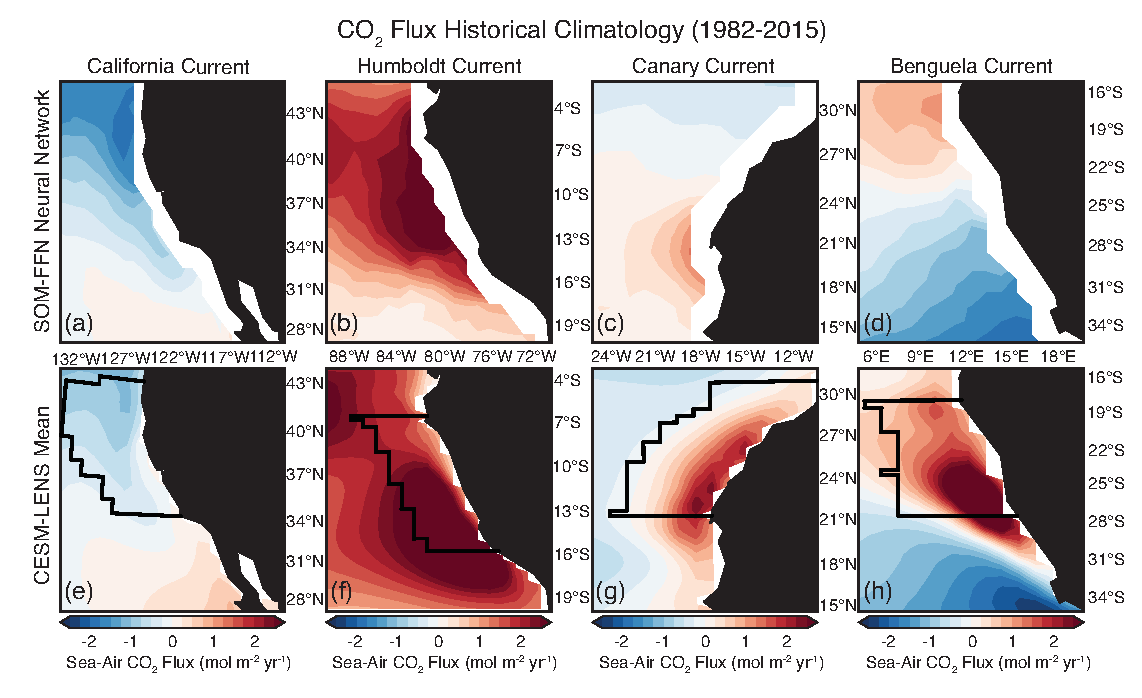
\includegraphics[width=12cm]{figures/figure1.eps}
\caption{Comparison of CO$_{2}$ flux climatology from 1982--2015 between the SOM-FFN (a--d) and the CESM-LENS (e--h). Red denotes outgassing of CO$_{2}$ from the ocean to the atmosphere, while blue represents uptake of CO$_{2}$ by the ocean. Black lines in e--h follow the model grid and show the region used in each EBUS for statistical analysis, which is based on the 10$^{o}$ latitude of most active upwelling from \citet{Chavez:2009} and confined to 800km offshore.}
\label{Fig:Eval}
\end{figure*}

\clearpage
\begin{figure*}[t]{}
	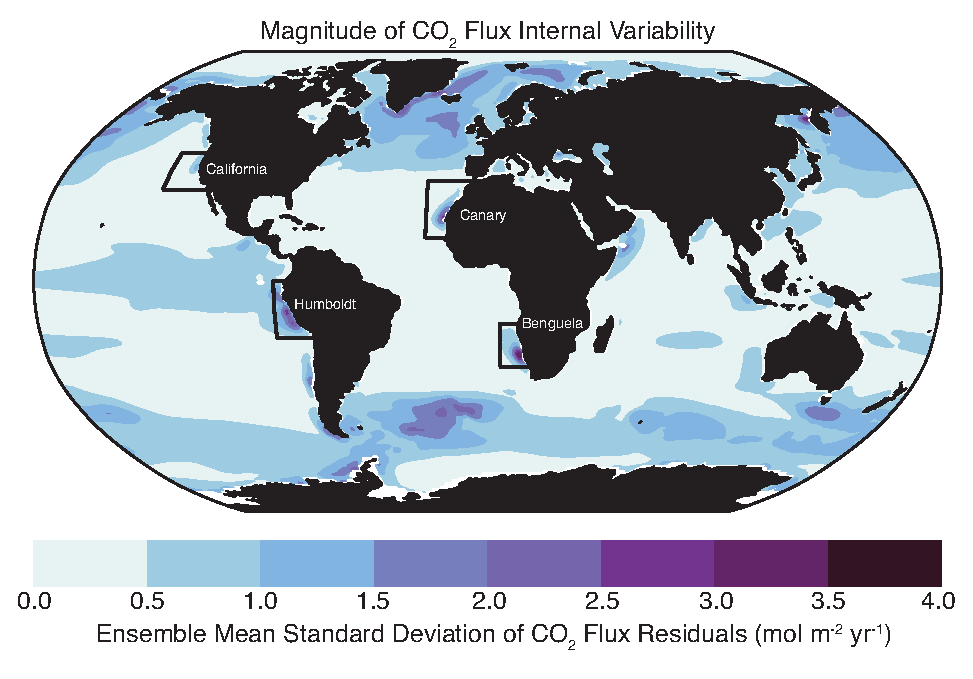
\includegraphics[width=12cm]{figures/figure2.eps}
	\caption{Magnitude of internal variability in CO$_{2}$ flux from 1920--2015 in the CESM-LENS. Residuals were generated by removing the ensemble mean -- which represents the seasonality and forced signal -- from each realization. Internal variability was then quantified by taking the ensemble mean standard deviation of the residuals from 1920--2015.}
	\label{Fig:Internal}
\end{figure*}

\clearpage
\begin{figure*}[t]
	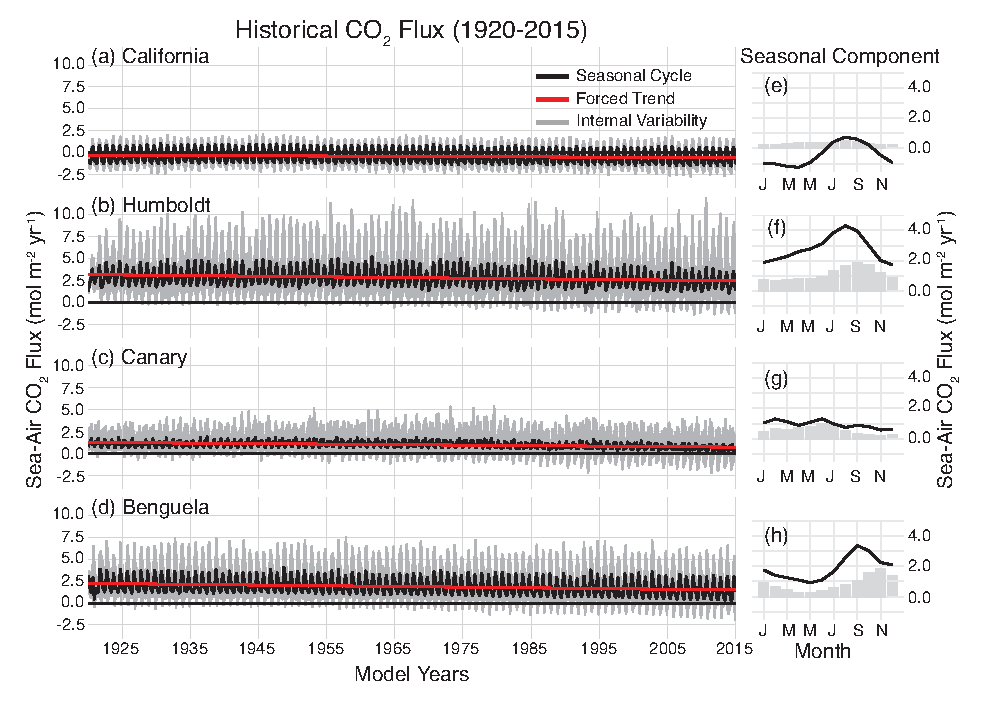
\includegraphics[width=12cm]{figures/figure3_with_seasonal_and_internal.eps}
	\caption{Time series of historical CO$_{2}$ flux (1920--2015) in the CESM-LENS for each of the four studied upwelling systems (a--d). The ensemble mean yields both the seasonal cycle (black) and the anthropogenic trend (red). Gray shading shows the bounds of the maximum and minimum realizations due to internal variability. Table~\ref{Table:1} displays the intercept, seasonality, internal variability, and anthropogenic trend for each system. Plots e--h show the mean seasonal cycle (black line) and ensemble mean monthly internal variability (gray bars) for 1920--2015 for each system.}
	\label{Fig:TimeSeries}
\end{figure*}

\clearpage
\begin{figure*}[t]
	\includegraphics[width=12cm]{figures/figure4-vert.eps}
	\caption{Correlations between area--weighted CO$_{2}$ flux residuals in the statistical study regions outlined in black in Figure~\ref{Fig:Eval} (e--g) and SSTa (a--b; California, Humboldt) and SLPa (c; Canary) grid cells globally. Brown colors indicate that positive values of SSTa/SLPa correlate with outgassing, and blue with uptake. Contour lines begin at $\pm$ 0.3 and progress in intervals of 0.1. Correlations were performed for each realization individually and the ensemble mean of those global correlations are presented here. Violin plots of correlations between area--weighted CO$_{2}$ flux residuals from (a--c) with major modes of Pacific (d--e) and Atlantic (f) variability.}
	\label{Fig:GlobalRegressions}
\end{figure*}

\clearpage
\begin{figure*}[t]
	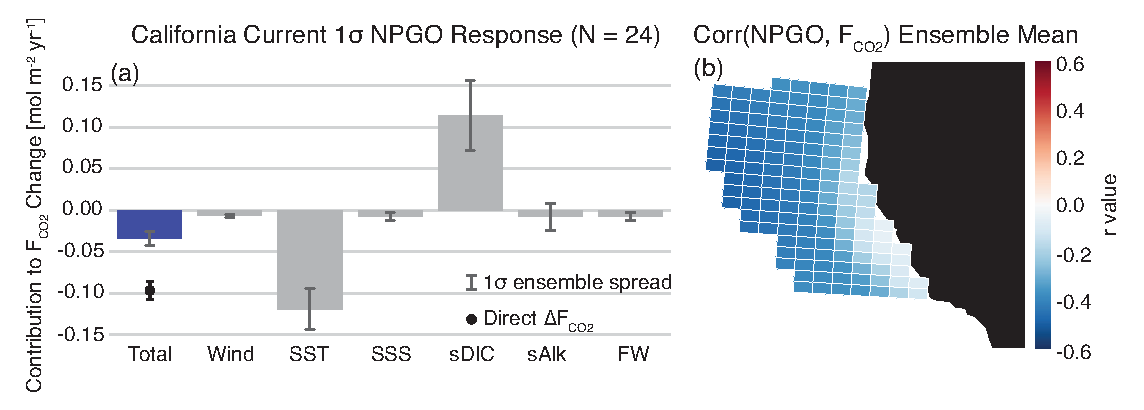
\includegraphics[width=12cm]{figures/figure5_notable.eps}
	\caption{Linear Taylor expansion from Eq. (4) for CalCS CO$_{2}$ flux residuals regressed onto the NPGO (a). Gray bars represent the ensemble mean contributions of each variable to the CO$_{2}$ flux anomaly. Error bars represent the one standard deviation spread of the full ensemble. The individual bars sum to the ``total" bar to approximate the direct regression of $\Delta F_{CO_{2}}$ onto the NPGO, which is denoted as the black dot with its associated ensemble spread. The ensemble mean grid cell correlations between CO$_{2}$ flux residuals and the NPGO in the CalCS study region are displayed in (b). Positive correlations are associated with outgassing, negative with uptake. Values and ensemble spread for each bar are presented in Table~\ref{Table:2}.}
	\label{Fig:CalDecompNPGO}
\end{figure*}

\clearpage
\begin{figure*}[t]
	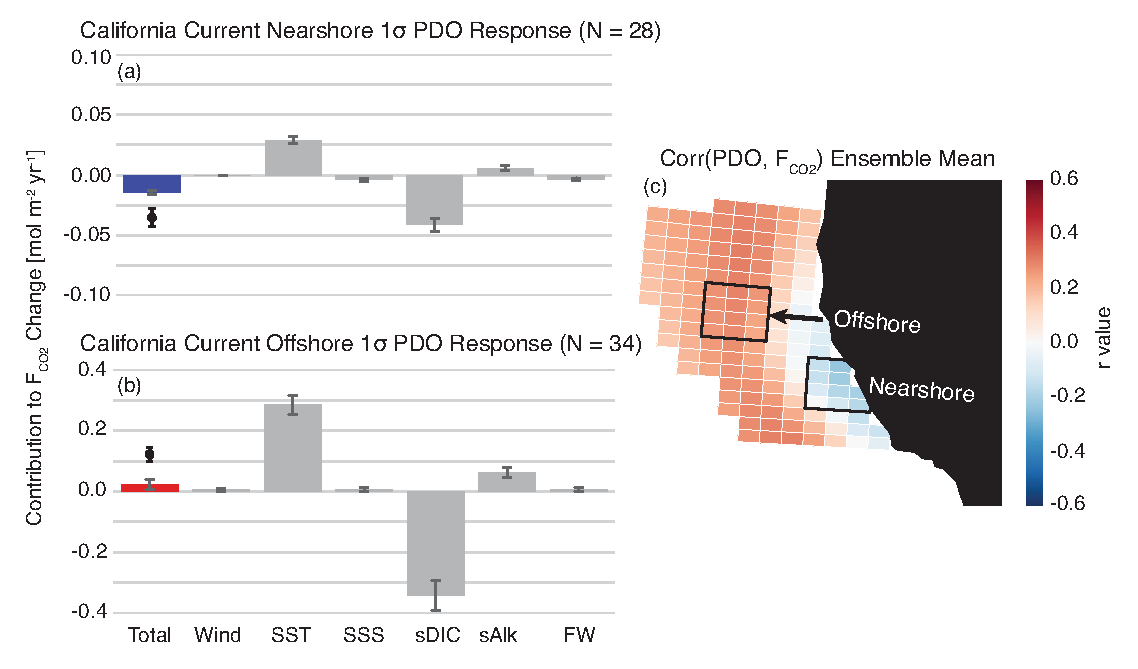
\includegraphics[width=12cm]{figures/figure6.eps}
	\caption{As in Figure~\ref{Fig:CalDecompNPGO}, but in response to the PDO for a nearshore region (a) and offshore region (b). Note that the offshore decomposition (b) has a y-axis range four times that of the nearshore decomposition (a).}
	\label{Fig:CalDecompPDO}
\end{figure*}

\clearpage
\begin{figure*}[t]
	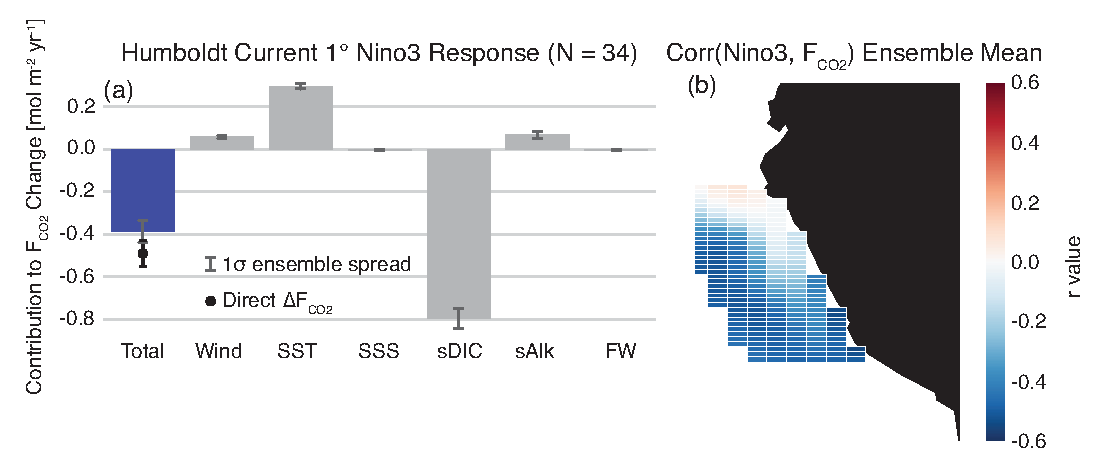
\includegraphics[width=12cm]{figures/figure7.eps}
	\caption{As in Figure~\ref{Fig:CalDecompNPGO}, but for the Humboldt Current response to the Nino3 index.}
	\label{Fig:HumDecompENSO}
\end{figure*}

\clearpage
\begin{figure*}[t]
	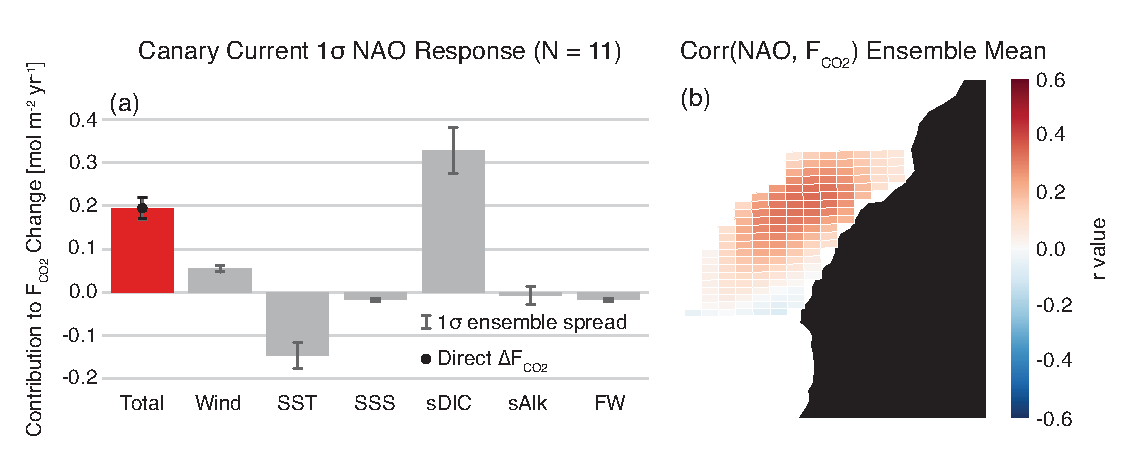
\includegraphics[width=12cm]{figures/figure8.eps}
	\caption{As in Figure~\ref{Fig:CalDecompNPGO}, but for the Canary Current response to the NAO.}
	\label{Fig:CanDecompNAO}
\end{figure*}

\clearpage
\begin{figure*}[t]
	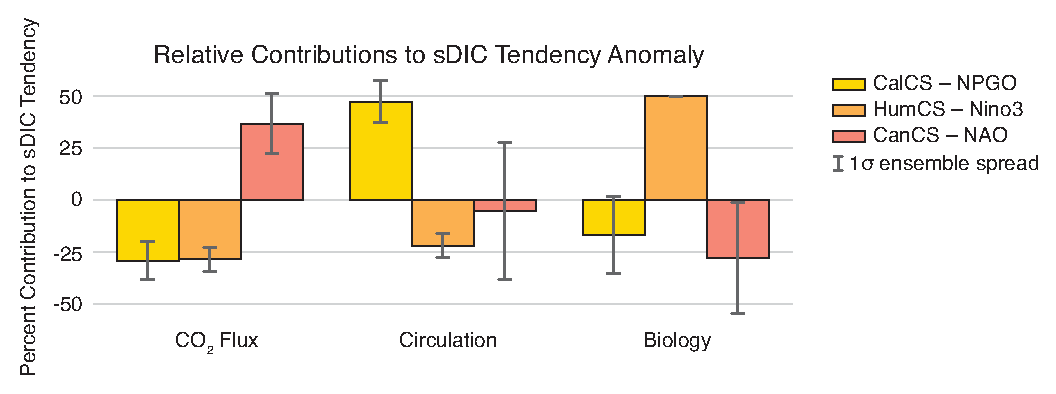
\includegraphics[width=12cm]{figures/figure9.eps}
	\caption{Relative contributions of anomalous CO$_{2}$ flux, physical circulation, and biology to the approximated sDIC tendency anomaly for the CalCS (yellow), HumCS (orange), and CanCS (red) in response to the NPGO, Nino3, and NAO, respectively. Error bars show the 1 standard deviation spread of the ensemble. For a given simulation, the absolute values of the three components sum to 100\%. These values were approximated using Equation 5.}
	\label{Fig:sDICDecomp}
\end{figure*}

\clearpage
\begin{figure*}[t]
	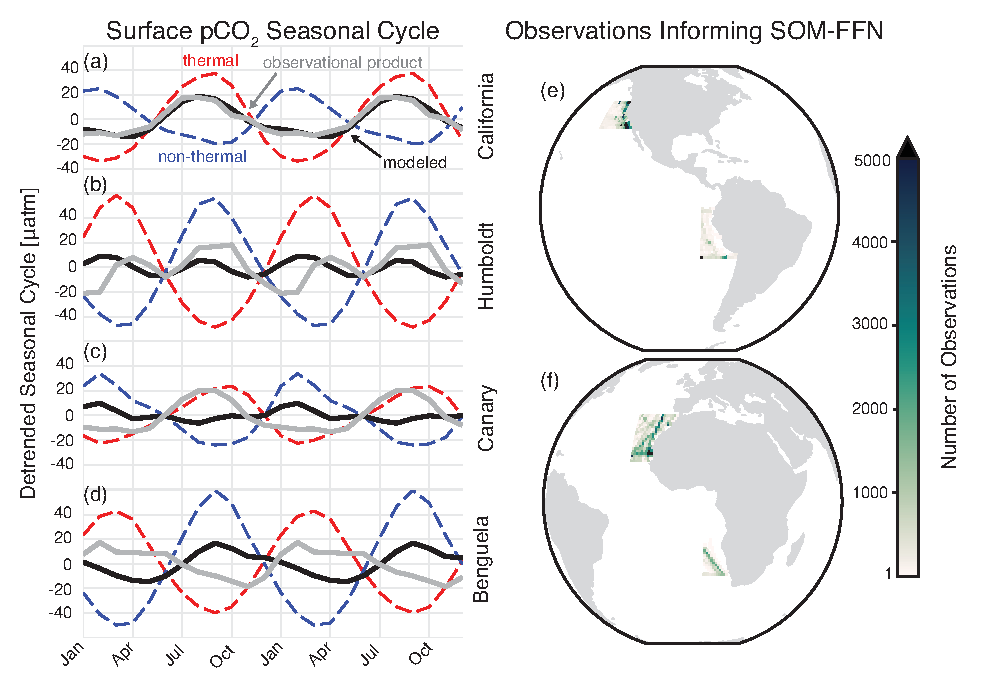
\includegraphics[width=12cm]{figures/seasonal_plot.eps}
	\caption{}
	\label{Fig:seasonal}
\end{figure*}


\clearpage
\begin{table}[t]
\caption{Statistics for CO$_{2}$ fluxes in the CalCS, HumCS, CanCS, and BenCS from 1920--2015. The seasonal component is computed as the standard deviation of the ensemble mean after removing a fourth-order polynomial fit to remove the anthropogenic trend. The internal component is computed as the ensemble mean standard deviation of the residuals. The trend is computed as the first-order ordinary least squares regression coefficient. The intercept is derived from this linear regression. The non-seasonal component represents the fraction of total variability (seasonal plus internal) to which the internal component contributes. The signal-to-noise ratio reflects the magnitude of the long-term trend relative to the magnitude of internal variability.}
\begin{adjustbox}{width=1\textwidth}
\begin{tabular}{l r r r r r r}
\tophline
Upwelling System & Intercept$^{1}$ & Seasonal$^{1}$ & Internal$^{1}$ & Trend$^{23}$ & Non-Seasonal Component ($\%$) & Signal-to-Noise \\
\middlehline
California (34$^{o}$ N--44$^{o}$ N) & -0.27 & 0.71 & 0.33 & -0.31 &  31 & 0.94 \\
Humboldt (16$^{o}$ S--6$^{o}$ S)  & 3.16 & 0.83 & 1.20 & -0.71 & 59 & 0.59 \\
Canary (21$^{o}$ N--31$^{o}$ N) & 1.23 & 0.23 & 0.62 & -0.56 & 73 & 0.90 \\
Benguela (28$^{o}$ S--18$^{o}$ S) & 2.25 & 0.77 & 0.98 & -0.76 & 56 & 0.78 \\
\bottomhline
\end{tabular}
\end{adjustbox}
\label{Table:1}
\belowtable{$^{1}$mol m$^{-2}$ yr$^{-1}$ \\
                       $^{2}$mol m$^{-2}$ yr$^{-1}$ 96yr$^{-1}$ \\
                   $^{3}$ All trends are significant to $\alpha$ = 0.05 for a one-sided Mann-Kendall Test}           
\end{table}


\clearpage
\begin{table}[ht]
	\caption{Estimated contributions to CO$_{2}$ flux anomalies, $\Delta F$ using Equation 4.}
	\begin{adjustbox}{width=1\textwidth}
	\begin{tabular}{l r r r r r}
		\tophline
		Quantity & CalCS -- NPGO  & CalCS -- PDOo & CalCS -- PDOn & HumCS -- Nino3 & CanCS -- NAO \\
		\middlehline
		\multicolumn{6}{c}{{\it Individual Terms}} \\
		$\frac{\partial F}{\partial U}\Delta U$ & -0.01 $\pm$ 0.0  & 0.01 $\pm$ 0.0 & 0.0 $\pm$ 0.0 & 0.06 $\pm$ 0.01  & 0.05 $\pm$ 0.01  \\
		$\frac{\partial F}{\partial T}\Delta T$ & -0.12 $\pm$ 0.02  & 0.28 $\pm$ 0.03 &0.03 $\pm$ 0.0 & 0.29 $\pm$ 0.01  &  -0.15 $\pm$ 0.03 \\
		$\frac{\partial F}{\partial S}\Delta S$ & -0.01 $\pm$ 0.0  & 0.01 $\pm$ 0.01 & 0.0 $\pm$ 0.0 & -0.0 $\pm$ 0.0  &  -0.02 $\pm$ 0.0 \\
		$\frac{S}{S_{0}}\frac{\partial F}{\partial DIC}\Delta sDIC$ & 0.11 $\pm$ 0.04  & -0.34 $\pm$ 0.05 & -0.04 $\pm$ 0.01 & -0.8 $\pm$ 0.05  & 0.33 $\pm$ 0.05  \\
		$\frac{S}{S_{0}}\frac{\partial F}{\partial Alk}\Delta sAlk$ & -0.01 $\pm$ 0.02 & 0.06 $\pm$ 0.02 & 0.01 $\pm$ 0.0 & 0.07 $\pm$ 0.01  &  -0.01 $\pm$ 0.02 \\
		$\frac{\partial F}{\partial fw}\Delta fw$ & -0.01 $\pm$ 0.0 & 0.01 $\pm$ 0.01 & 0.0 $\pm$ 0.0 & 0.0 $\pm$ 0.0  &  -0.02 $\pm$ 0.0 \\
		\multicolumn{6}{c}{{\it Sum of Terms Versus Modeled}} \\
		$\Sigma$ & -0.03 $\pm$ 0.01 & 0.02 $\pm$ 0.02 & -0.01 $\pm$ 0.0 & -0.38 $\pm$ 0.05 & 0.21 $\pm$ 0.03 \\
		$\Delta F_{mod}$ & -0.10 $\pm$ 0.01 & 0.12 $\pm$ 0.02 & -0.04 $\pm$ 0.01 & -0.49 $\pm$ 0.06 & 0.2 $\pm$ 0.02 \\
		\bottomhline
	\end{tabular}
	\end{adjustbox}
\label{Table:2}
\end{table}

\clearpage
\begin{table}[t]
	\caption{Regression coefficients between the given EBUS and climate index for anomaly time series of the estimated contributions toward the sDIC tendency integrated over the upper 100m and the total surface area of the system, as in Equation 5.$^{1}$}
		\begin{tabular}{l l l l}
			\tophline
			Term & CalCS -- NPGO & HumCS -- Nino3 & CanCS -- NAO \\
			\middlehline
			$\frac{dsDIC^{\prime}}{dt}$ & 0.003 $\pm$ 0.001 & -0.010 $\pm$ 0.002 & 0.004 $\pm$ 0.001 \\
			$J^{\prime}_{ex}$  & -0.076 $\pm$  0.020 & -0.484 $\pm$ 0.061 & 0.051 $\pm$ 0.021 \\
			$J^{\prime}_{bio}$ & -0.068 $\pm$ 0.048 & 0.861 $\pm$ 0.081 & -0.049 $\pm$ 0.054 \\
			$J^{\prime}_{circ}$ & 0.147 $\pm$ 0.064 & -0.387 $\pm$ 0.128 & 0.002 $\pm$ 0.056 \\
			\bottomhline
		\end{tabular}
	\label{Table:3}
	\belowtable{$^{1}$Units are GgC~yr$^{-1}$}     
\end{table}

\end{document}
